
% PREÁMBULO*******************************************

\documentclass[a4paper,twocolumn]{article}

\usepackage[utf8]{inputenc}
\usepackage{authblk}
\usepackage[spanish,es-tabla]{babel}
% \usepackage[top = 2cm, bottom = 2cm, left = 2.5cm, right = 2.5cm]{geometry}
\usepackage{amsmath,amsthm,amssymb,amsbsy,bm}
\usepackage{graphicx} % Nos permite insertar figuras
\usepackage{subfigure} % Nos permite redimensionar tablas
\usepackage{booktabs}
\usepackage[usenames]{color} % Nos permite incoporar color a los textos
\usepackage[pdftex]{hyperref} % Incluye hipervinculos en las referencias
\usepackage{comment} % Para insertar comentarios con \begin{comment} y \end{comment} Ojo!!! Han de ir solos en sus líneas, al principio total de la línea y sin nada después!!!
\usepackage{appendix}

\hypersetup{colorlinks=true,linkcolor=black, citecolor=black} % Quita el cuadradito del hipervinculo y cambia el color a negro, tanto en referencias a ecuaciones/tablas como en las referencias bibliográficas.

\usepackage{babelbib} % Para tener la bibliografia en castellano

\usepackage{soul} % Para dar formatos, por ejemplo poder usar \ul{} para subrayar

% Declaracion de nuevos entornos y comandos

\newtheorem*{keywords*}{Palabras Clave}

% Titulo, autores, datos de afiliacion y fecha

\title{Reflexión y refracción de la luz}
\author{Zigor Marroquín Martínez}
\affil{zmarroqui1@alumno.uned.es}
\date{} % Indicarlo asi si no queremos que aparezca la fecha


% CUERPO**********************************************

\begin{document}
	
	\maketitle
	
	\begin{abstract}
		
		La reflexión y la refracción de la luz son dos fenómenos muy `cercanos' y dependientes. Aparecen en el momento en el que un rayo de luz cambia de medio, y que aparezca uno u otro, o los dos a la vez, depende por un lado de los dos medios que toman parte en el proceso, y por otro del ángulo con que incide el rayo respecto a la normal al plano de cambio de medio. La óptica estudia la relación entre los ángulos que forman el rayo incidente, el reflejado y el refractado (de haberlo) con la normal a la superficie de separación de los dos medios. % \textcolor{red}{REFERENCIAS (bibliografía). Citar tablas/figuras para entendernos. Ordenarlo todo un poco mejor???}
		
		\begin{keywords*}
			
			Reflexión, refracción, Ley de Snell, aproximación de Gauss, ángulo límite.
			
		\end{keywords*}
		
	\end{abstract}
	
	\section{Introducción}

         % Breve resumen que justifique la elaboración de la practica, y su propósito. Se deben incluir las bases teóricas.
         
        Las leyes de la reflexión y la refracción de la luz se conocen desde la antigüedad, pero no fueron establecidas matemáticamente hasta que Descartes y Newton las publicaron en sus tratados de óptica \cite{newton1952opticks} \cite{descartes1664monde}.
        
        Posteriormente, el matemático holandés Willebrord Snel van Royen enunció la ley que lleva su nombre (\textit{Ley de Snell}) \cite{huygens1703dioptrica}, relacionando los senos de los ángulos de incidencia y refracción de la luz al cambiar de medio. La aproximación paraxial o de Gauss la simplifica para ángulos pequeños.
        
        Estos enunciados se basan en relaciones matemáticas sencillas, y que pueden comprobarse además con dispositivos experimentales simples. Éste es el objetivo de esta práctica.



 
	\section{Fundamento teórico} \label{cap:FunTeo}

        % Desarollar la teoría relacionada con el procedimiento experimental. Sin copiarla literalmente del guión. Expresar los términos físicos con corrección. No muy larga, resumen de los contenidos teóricos básicos.
        
        La práctica tomará como base los principios básicos de la óptica.
        
        Por un lado, las leyes de la reflexión y la refracción de la luz:
        
        \begin{itemize}
        
            \item El rayo incidente, el rayo reflejado, el rayo refractado y la normal a la superficie que separa los dos medios implicados están en un mismo plano, que se denomina \textit{plano de incidencia}.
            
            \item Los ángulos de incidencia y de reflexión son iguales (\textit{ley de la reflexión}):     
                \begin{equation}
                    \theta_i = \theta_r
                \end{equation}
                
            \item El seno del ángulo de refracción es proporcional al seno del ángulo de incidencia (\textit{ley de la refracción} \cite{huygens1703dioptrica}):            
                \begin{equation}
                    \sin \theta_t = \frac{1}{n} \sin \theta_i
                \end{equation}            
            donde $n$ es el \textit{índice de refracción del medio}, y cuyo valor es el cociente entre la velocidad de la luz en el medio de donde proviene y la velocidad de la luz en el medio a donde se transmite:            
                \begin{equation*}
                    n = \frac{c_1}{c_2}
                \end{equation*}
            
            \item Las leyes de la reflexión y la refracción son reversibles. Es decir, las direcciones de incidencia/reflexión y de incidencia/refracción son intercambiables, y las leyes se siguen cumpliendo.
            
            Debido a esto, cuando la luz pasa de un medio de índice de refracción absoluto mayor a otro de índice menor, y a partir de cierto ángulo de incidencia, se produce el fenómeno de la \textit{reflexión total} (no hay refracción). Este ángulo de incidencia se conoce como \textit{ángulo límite}. 
            
        \end{itemize}

        Por otro lado, se utilizará también la llamada \textit{aproximación paraxial o de Gauss}, que es la aproximación de la ley de Snell para ángulos pequeños.
        
        Dado que para ángulos pequeños el seno, la tangente y el propio ángulo (expresado en radianes!) tienen prácticamente el mismo valor, puede considerarse:        
            \begin{equation}
                \theta_t = m \theta_i
            \end{equation}



            
        
	\section{Dispositivo experimental}
	
	Se realizarán dos montajes similares, aprovechando las capacidadades del laboratorio para poder realizar la práctica tanto con una `cubeta' (semicilindro) de vidrio como con una cubeta de agua. 
        
        \subsection{Montajes experimentales}

        % Cómo es el(los) montaje(s) experimental(es). Qué se pretende medir. Esquema(s). Foto(s).
        
        Ambos montajes serán iguales, simplemente uno de ellos utilizará una cubeta de vidrio y el otro una cubeta llena de agua.
        
        Como el objetivo del montaje es permitir la medición de los ángulos de los diferentes rayos, se colocará sobre la mesa una plancha base que tenga graficada una regla angular.
        
        Sobre la plancha, y con mucha precisión, se colocará primero la cubeta de vidrio y posteriormente la de agua. Es muy importante que las cubetas se encuentren perfectamente centradas y alineadas con los ejes horizontal y vertical de la regla.
        
        Por último, se conecta la caja de láseres a la red eléctrica, y se van buscando los ángulos de incidencia necesarios para ir realizando el análisis de la reflexión y refracción pedido por la práctica (ver figura \ref{fig:MonExpAirVid}).
        
        
        \begin{figure}[h!]
            \centering
            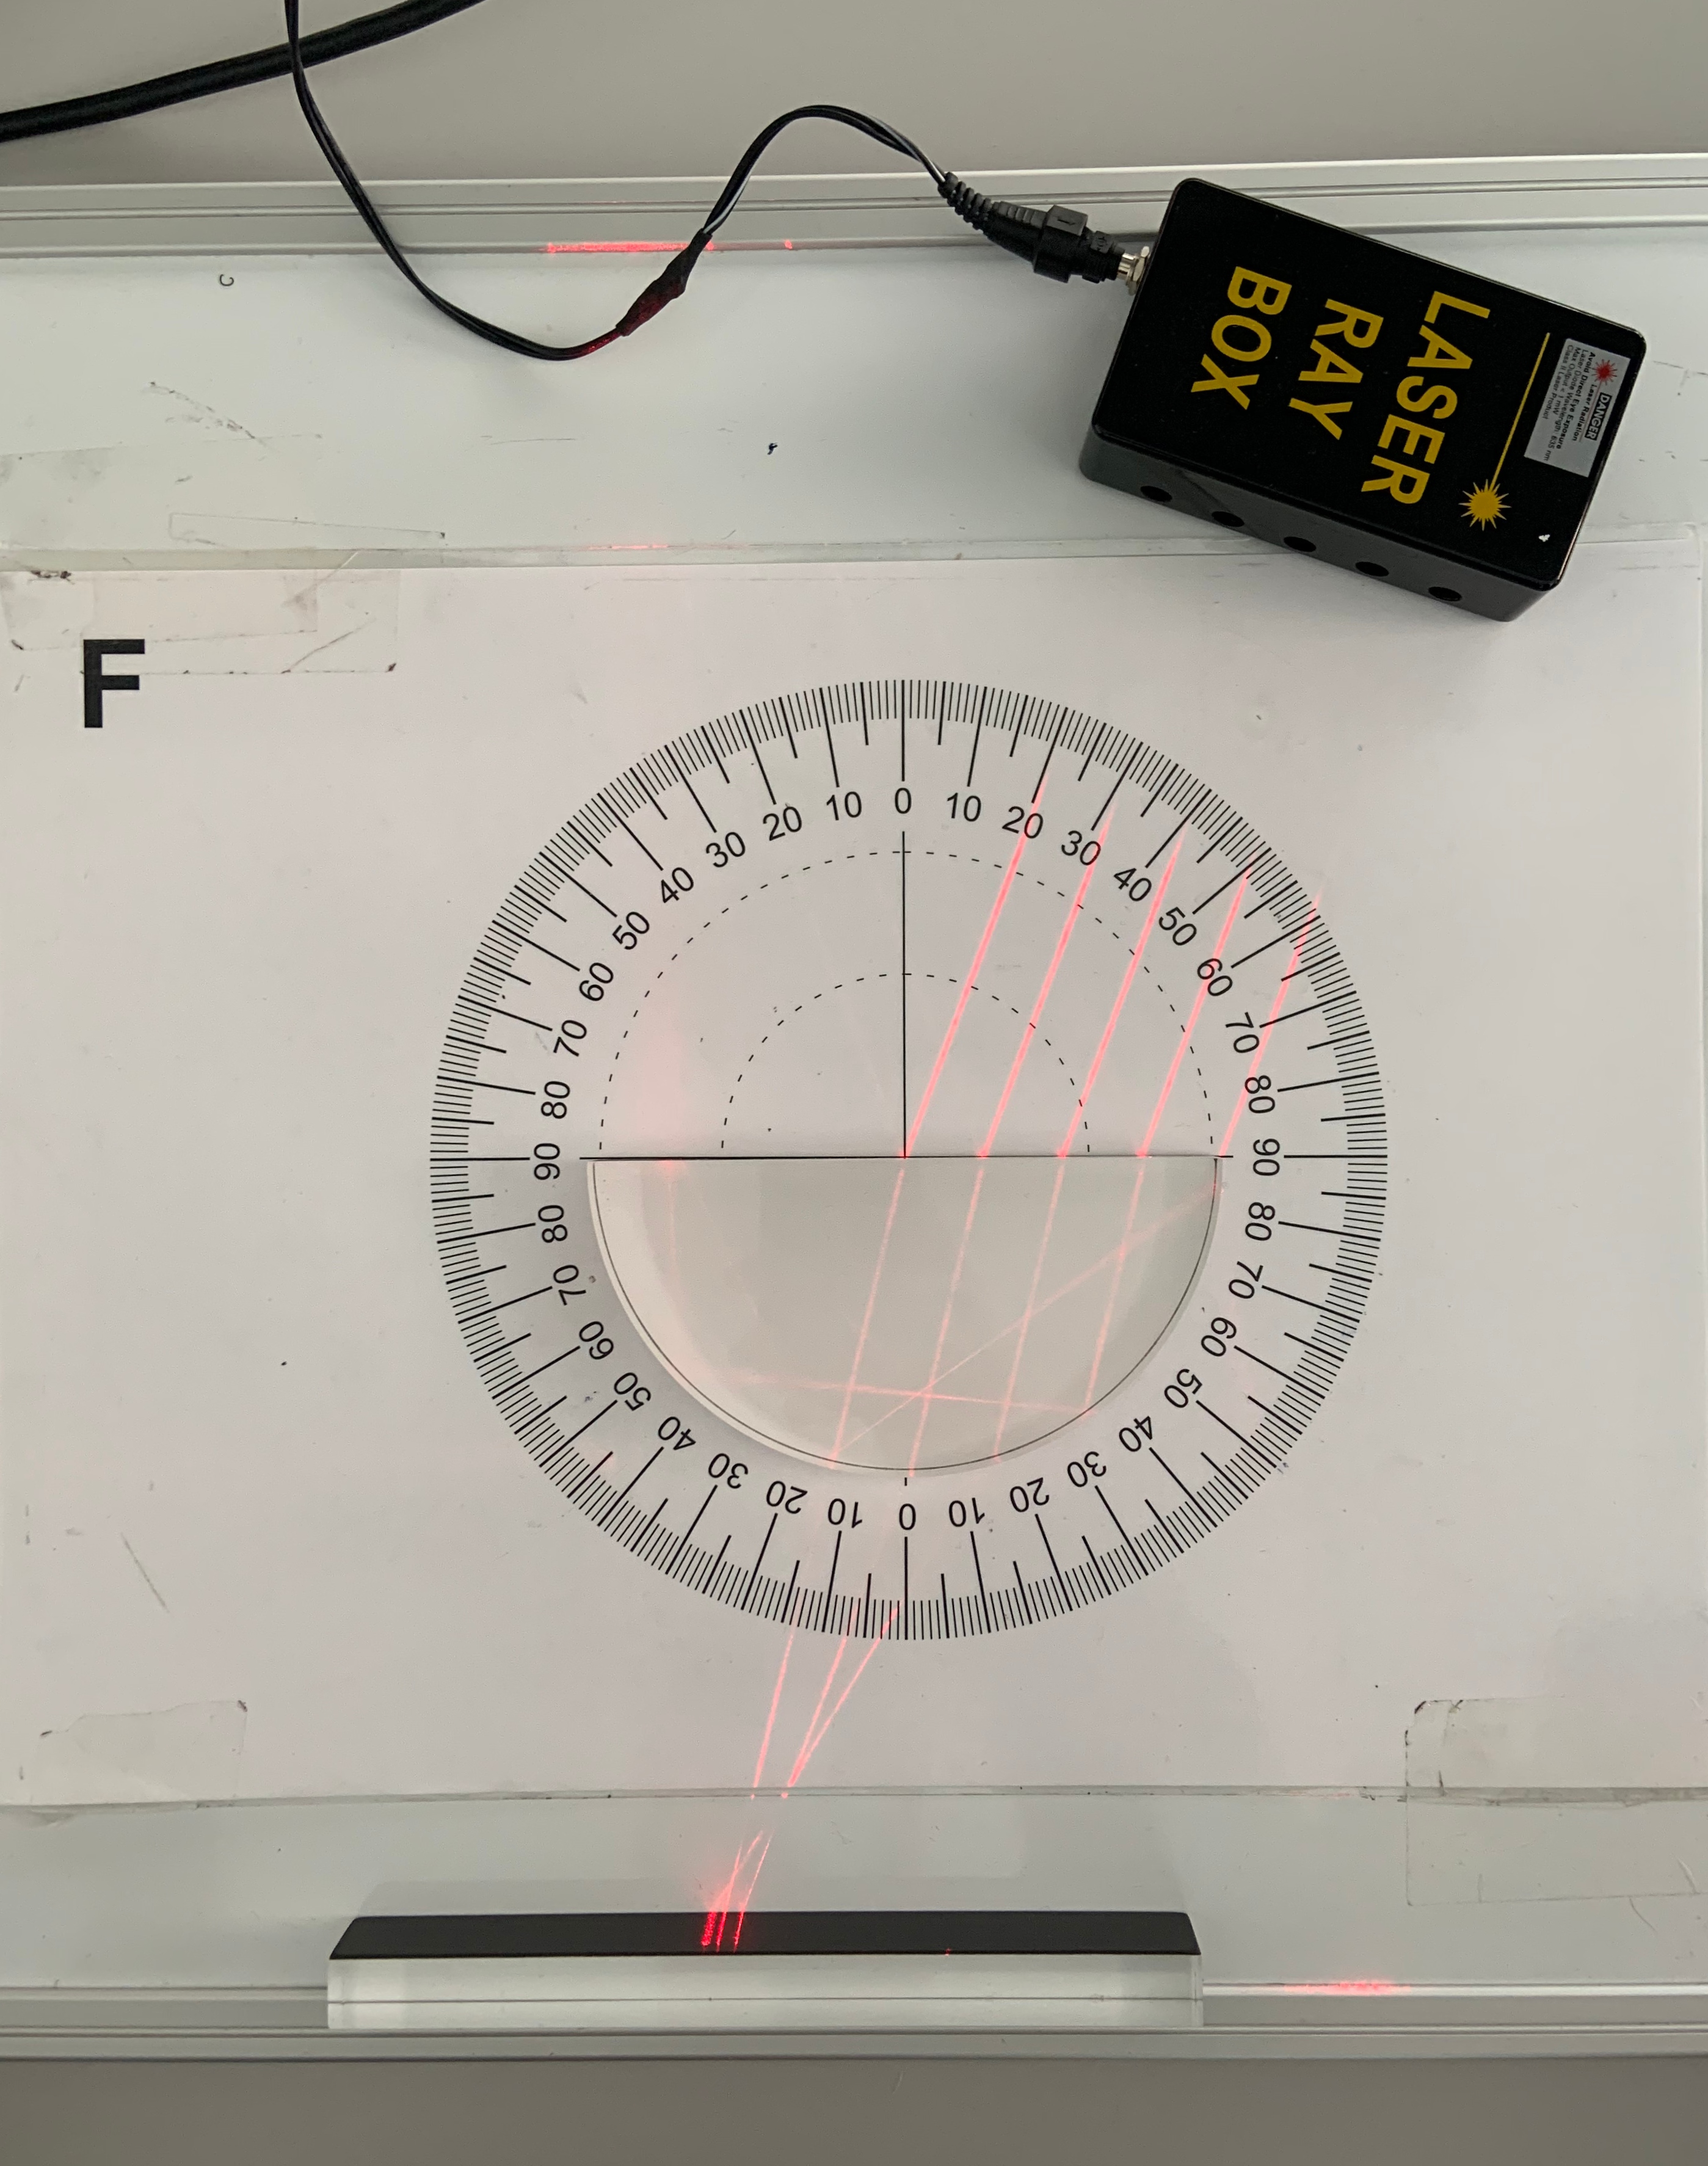
\includegraphics[width = 0.9\linewidth]{Fotos/Montaje experimental vidrio.jpg}
            \caption{Montaje experimental aire-vidrio.}
            \label{fig:MonExpAirVid}
        \end{figure}

\begin{comment}
        \begin{figure}[h!]
            \centering
            \includegraphics[width = 0.9\linewidth]{Fotos/Montaje experimental agua.jpg}
            \caption{Montaje experimental aire-agua.}
            \label{fig:MonExpAirAgu}
        \end{figure}
\end{comment}

        \subsection{Material empleado}
        
        % Listar material empleado. Describirlo. Analizar el error cometido en cada medida con cada uno de los aparatos. Fotos.
        
        Se describen con más detalle a continuación los elementos empleados para la instalación de los montajes descritos:
        
        \begin{itemize}
            \item \textbf{Plancha con regla angular:} plancha de plástico, tamaño aproximado DIN A3, con una regla angular impresa en su parte central. También dispone de unos ejes horizontal y vertical que permitirán por un lado alinear la cubeta y por el otro localizar el centro del sistema, que será donde deban incidir los rayos que se quieren estudiar.
            
            Las subdivisiones más pequeñas de la regla son de 1\textdegree. Se tomará como error de este instrumento de medida $\pm 1$\textdegree.

\begin{comment}
            \begin{figure}[h!]
                \centering
                \includegraphics[width = 0.9\linewidth]{Fotos/Plancha con regla.jpg}
                \caption{Plancha base con regla angular.}
                \label{fig:PlaBasRegAng}
            \end{figure}    
\end{comment}        

            \item \textbf{Cubetas de vidrio y agua:} son dos elementos algo diferentes: la mal llamada \textit{cubeta de vidrio} será un semicilindro macizo de vidrio, con base semicircular y una altura de unos tres centímetros; en cambio, la bien llamada \textit{cubeta de agua} tendrá una geometría similar pero fabricada en plástico y con el interior hueco, de manera que podrá llenarse de agua (ver figura \ref{fig:CubVidAgu}).
            
            El error asociado a ambas cubetas dependerá fundamentalmente de la precisión de su posicionamiento sobre la regla angular. La cubeta de agua introducirá además el error debido a la interfase de plástico que habrá entre los materiales aire-agua cuya óptica se quiere estudiar.

            \begin{figure}[h!]
                \centering
                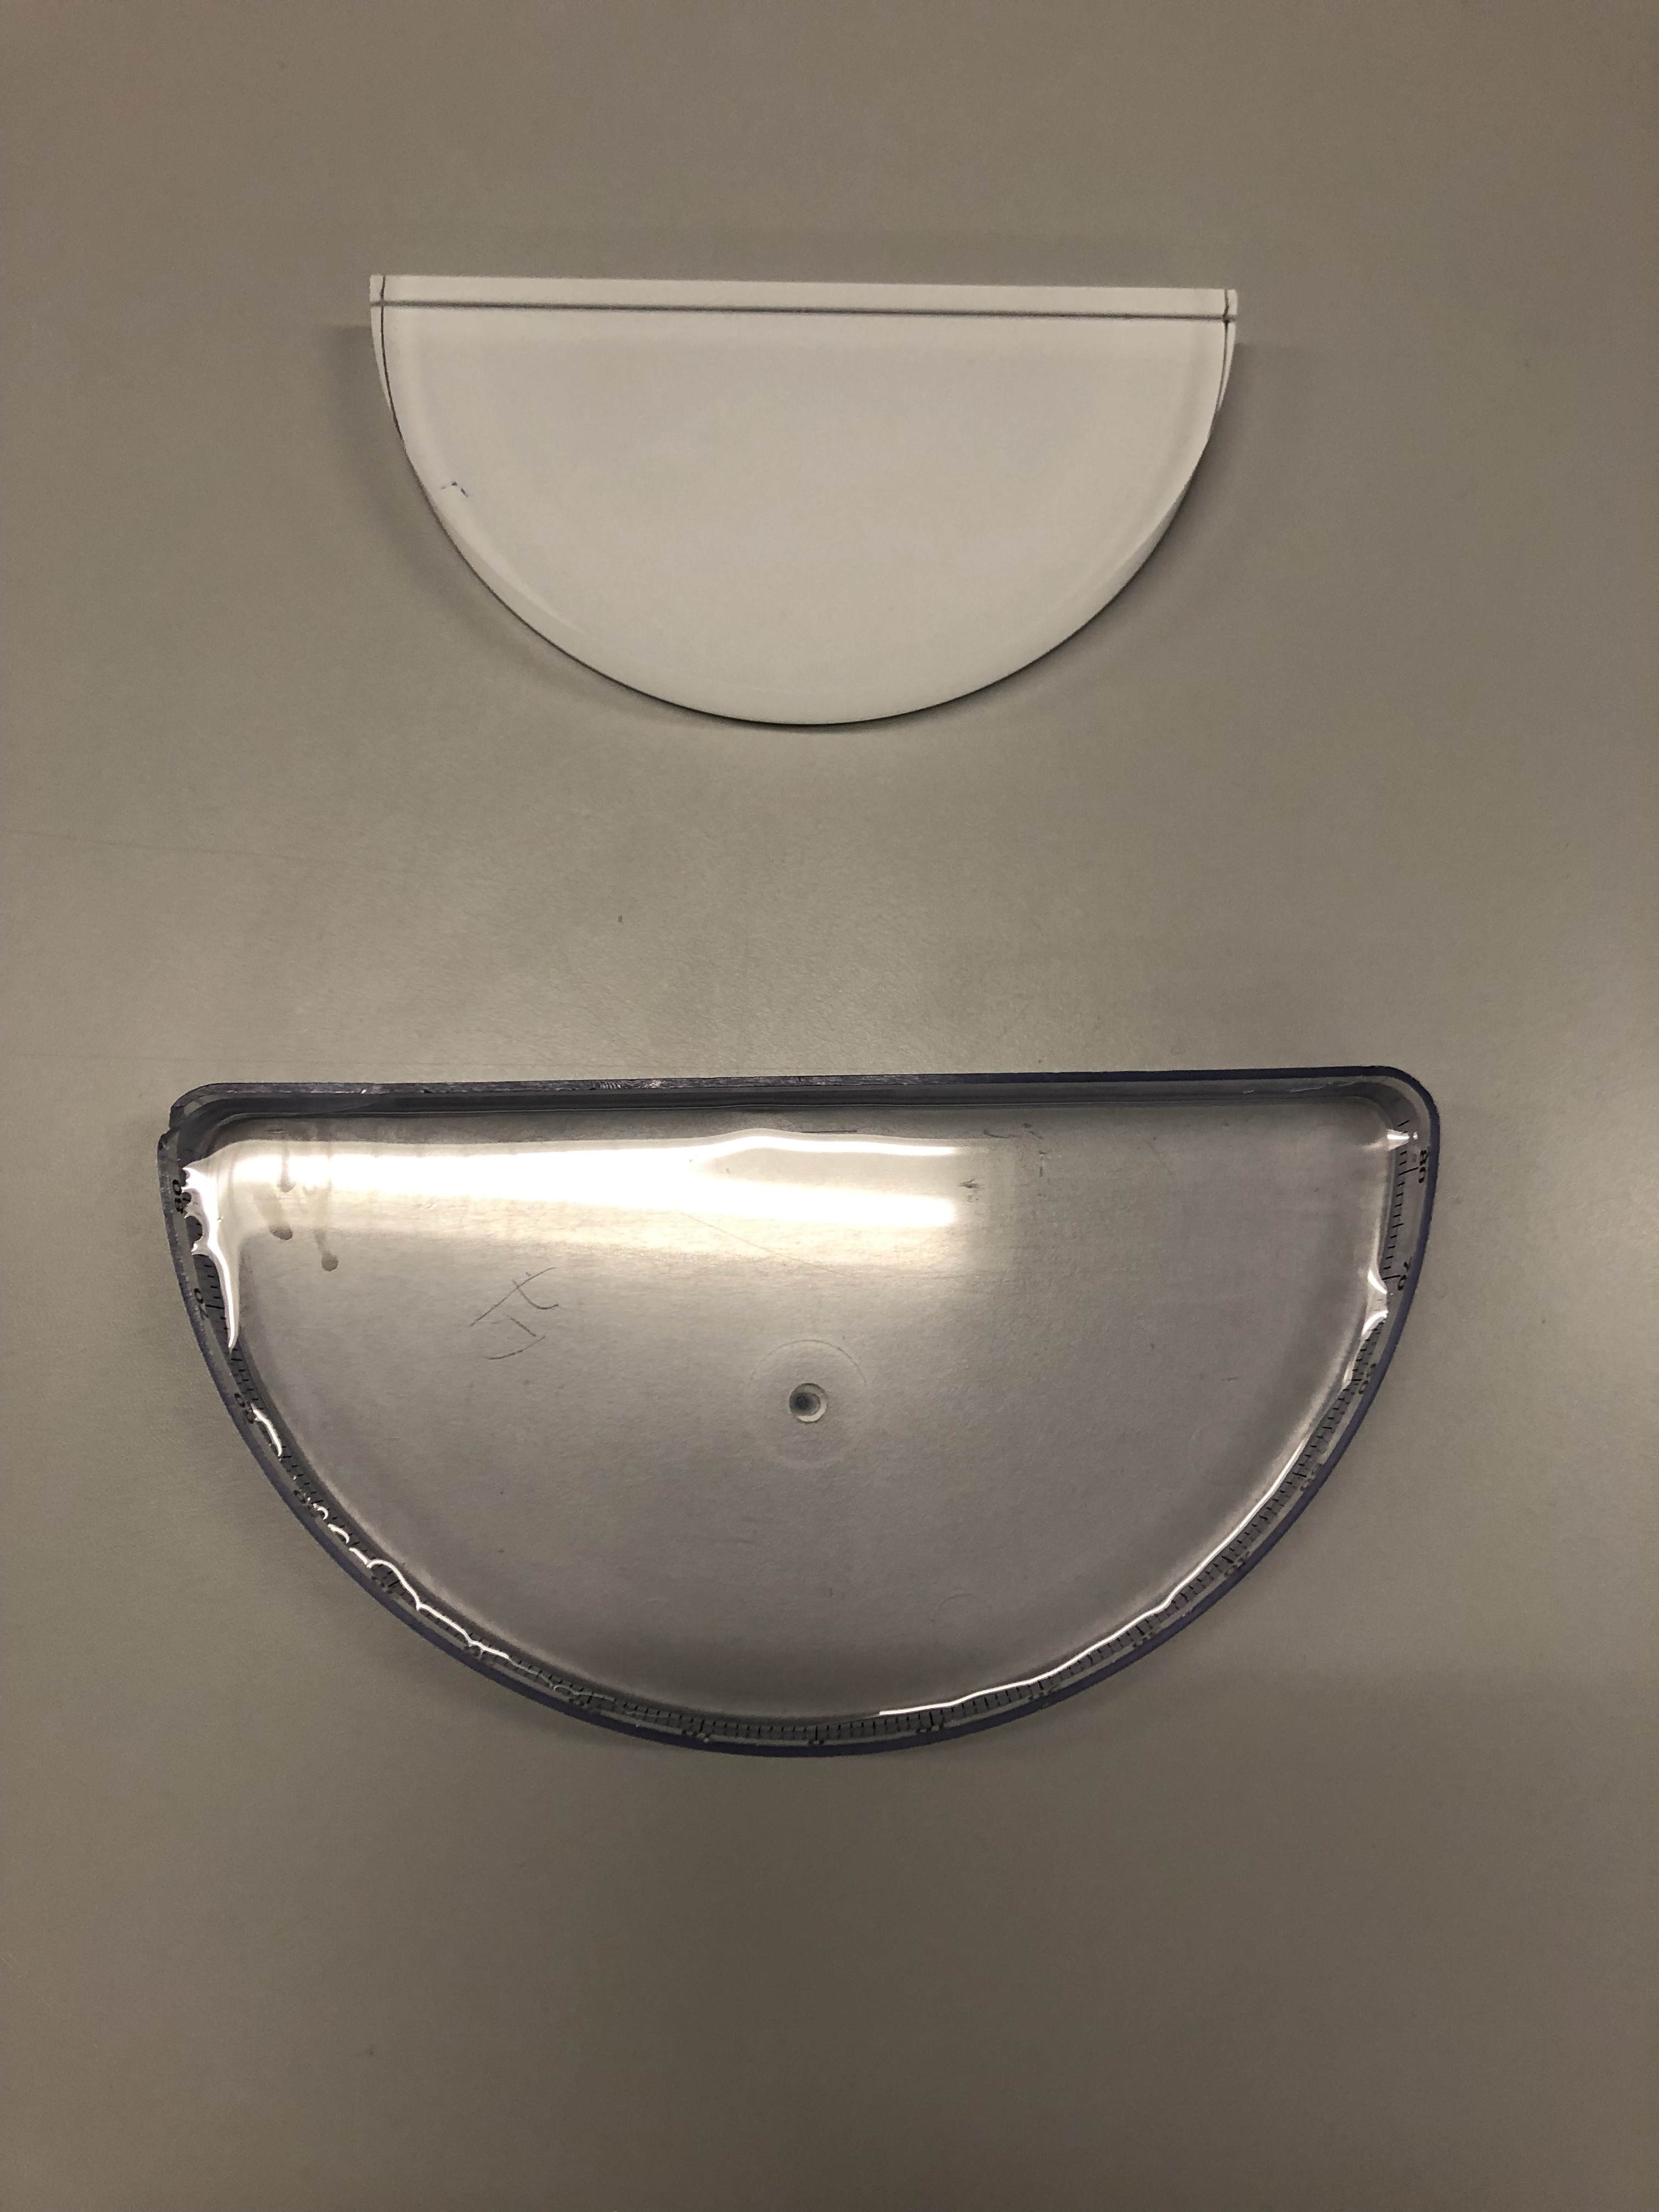
\includegraphics[width = 0.9\linewidth]{Fotos/Cubetas vidrio y agua.jpg}
                \caption{Cubeta de vidrio y cubeta de agua.}
                \label{fig:CubVidAgu}
            \end{figure}
            
            \item \textbf{Caja de láseres:} se trata de un láser de He-Ne de unos pocos miliwatios de potencia. Lanza cinco rayos paralelos al mismo tiempo (ver figura \ref{fig:CajLas}).
            
            El error asociado a este instrumento es el diámetro de los rayos, que se estima en torno a un 1 mm.

            \begin{figure}[h!]
                \centering
                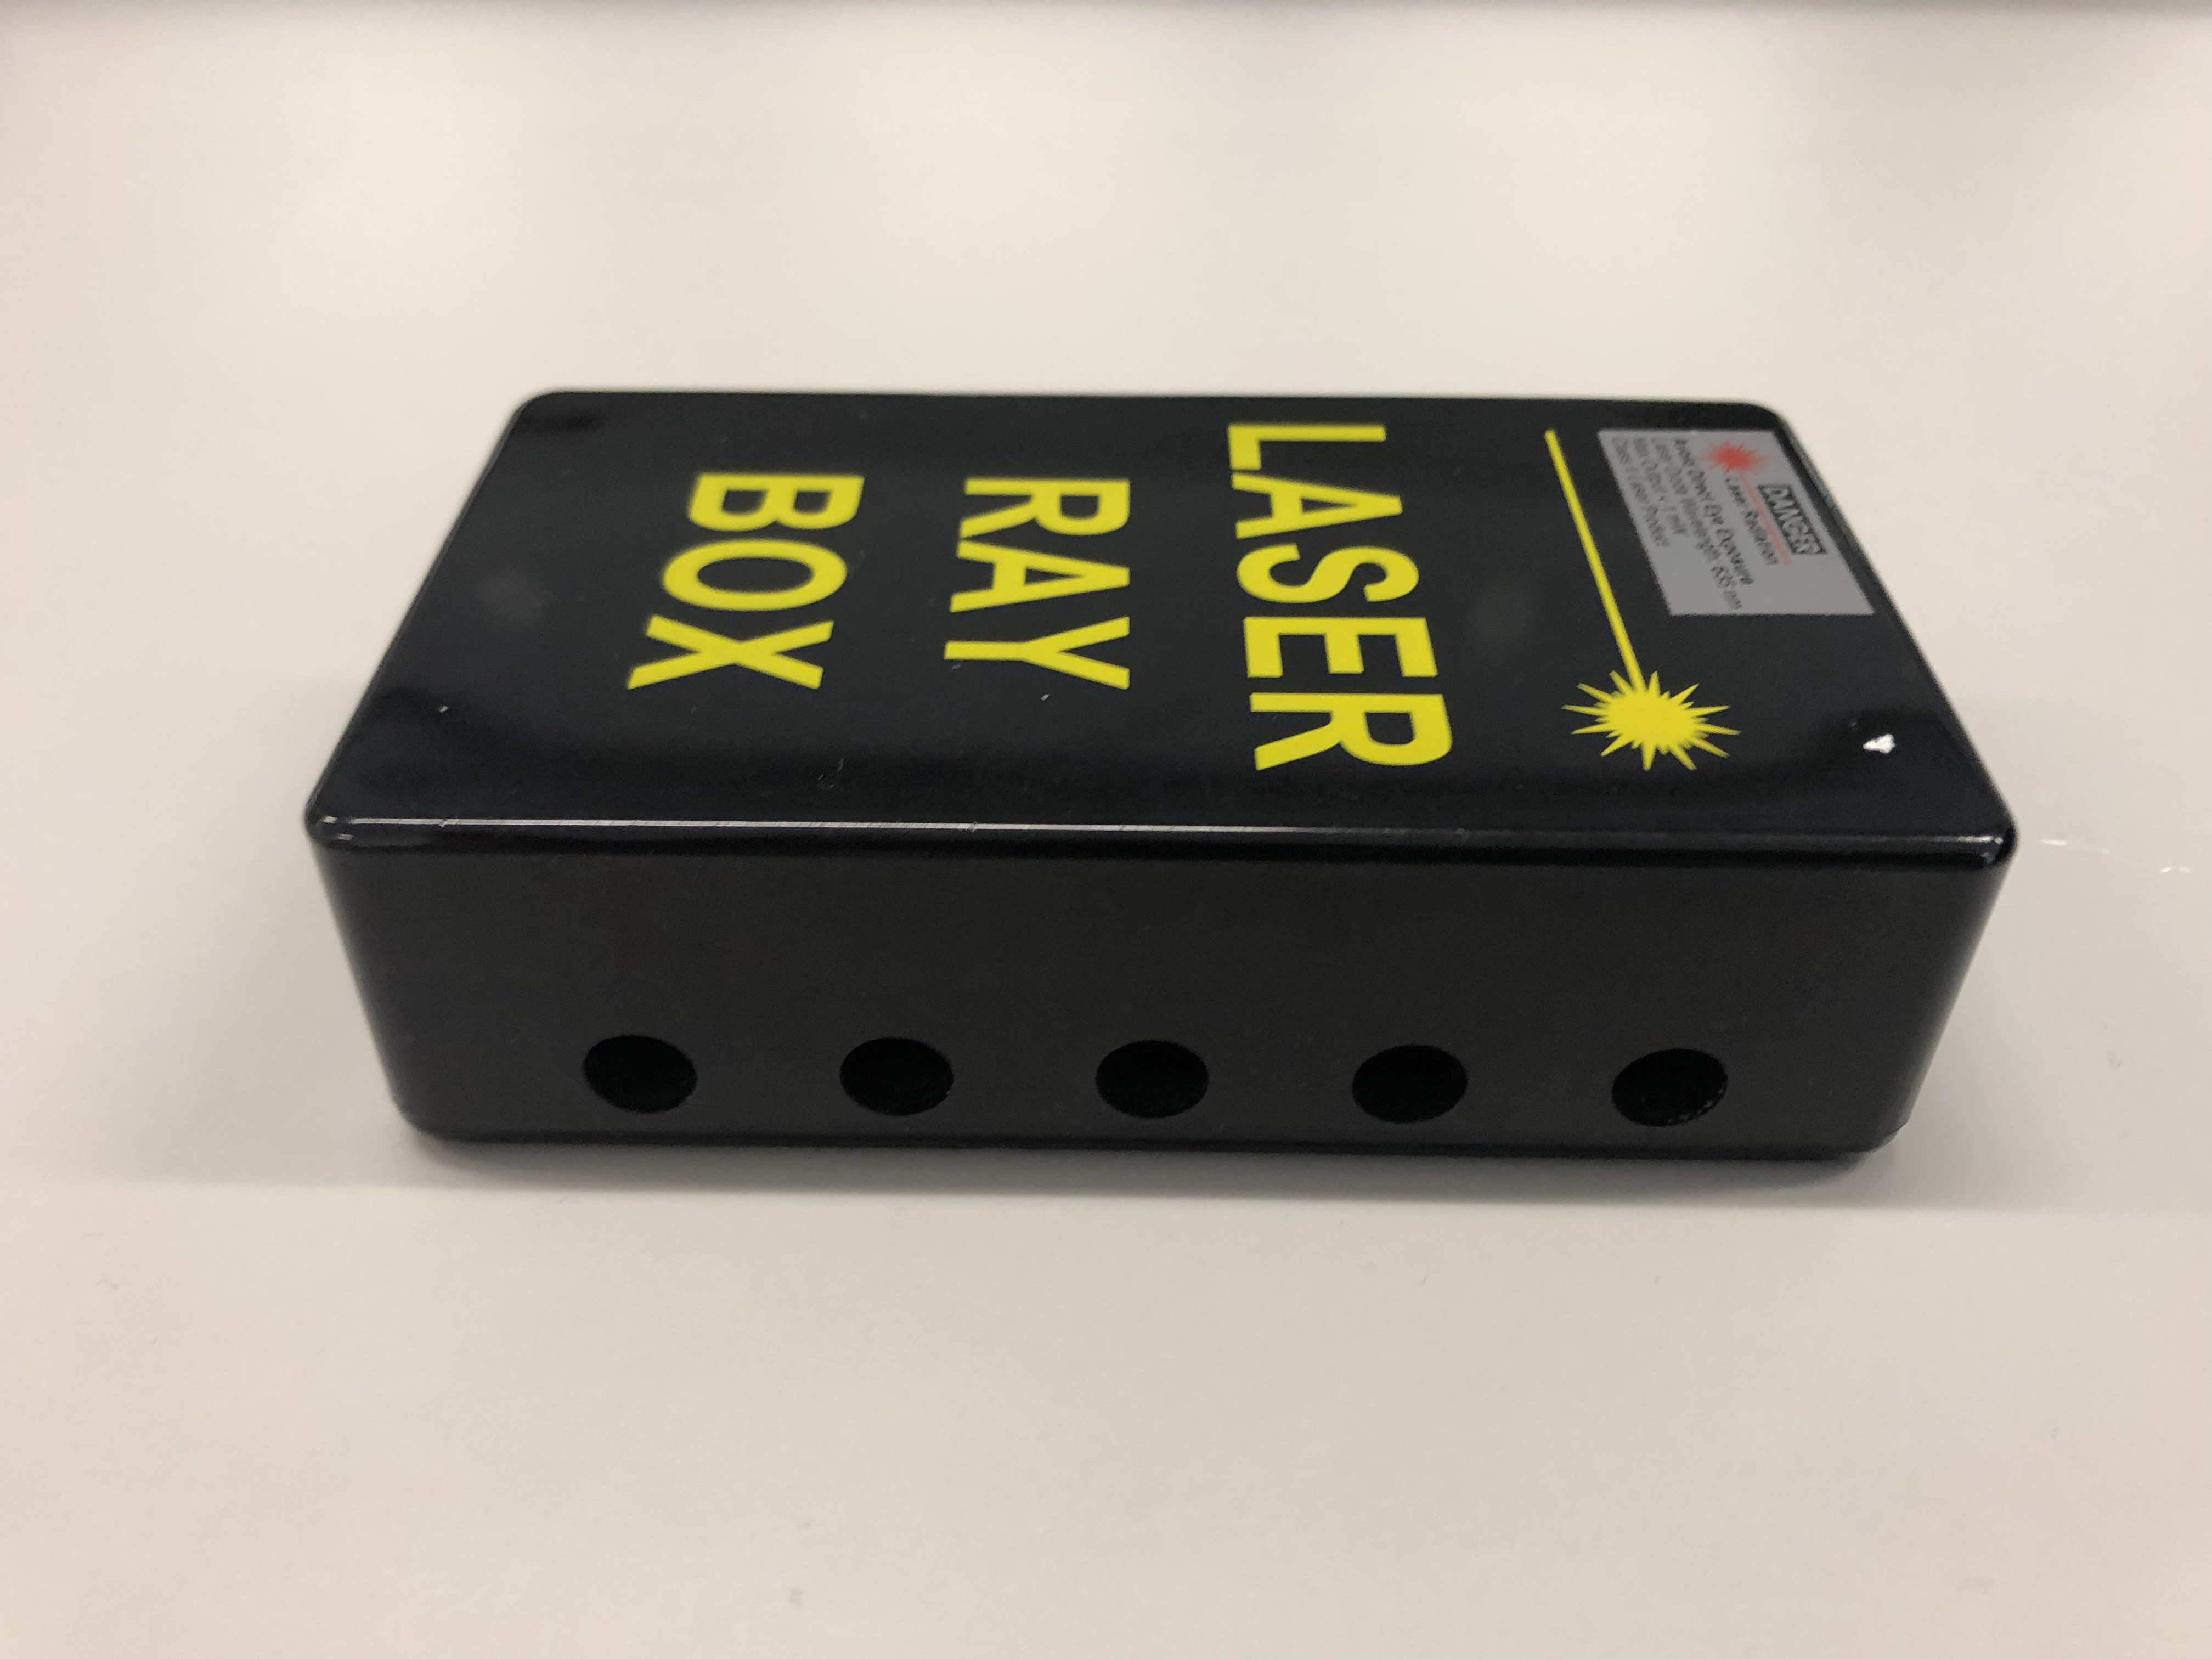
\includegraphics[width = 0.9\linewidth]{Fotos/Laser box.jpg}
                \caption{Caja de láseres.}
                \label{fig:CajLas}
            \end{figure}

        \end{itemize}




 
	\section{Procedimiento y resultados}

    % Explicar cómo se han tomado los datos. Resumirlos en tablas.
    
    % Mostrar los resultados en tablas y gráficas.
    
    % Explicar cómo se calculan los errores.
    
    Se realizan tres experimentos diferentes, y con ambas cubetas, para comprobar la validez de las leyes descritas en el apartado \ref{cap:FunTeo}.
    
        \subsection{Comprobación de que los tres rayos y la normal están en el mismo plano}
        
            Se hace incidir el láser en una dirección cualquiera y sobre cualquier punto de la superficie de separación aire-vidrio y aire-agua.
            
            Se comprueba que, tanto para la cubeta de vidrio como para la cubeta de agua, los rayos incidente, reflejado y refractado se encuentran siempre en un plano horizontal paralelo a la mesa. Esto implica que la recta normal a la superficie de separación en el punto de incidencia también pertenece a ese mismo plano.
    
        \subsection{Estudio de las relaciones entre los ángulos de incidencia, reflexión y refracción}

            Se realizan cuatro tareas diferentes para relacionar los tres rayos estudiados.
    
        \subsubsection{Medida de los ángulos de incidencia, reflexión y refracción} \label{cap:MedAngIncReflRefr}
        
            Se monta el dispositivo experimental, primero con la cubeta de vidrio y después con la cubeta de agua. Se comienza a lanzar rayos con el láser, asegurando que el punto de incidencia con la cubeta sea justo el centro de la misma.
            
            El ángulo de todos los rayos se mide siempre respecto a la normal. Se tomarán medidas para rayos incidentes de 5 a 85\textdegree.
            
            Los resultados obtenidos se presentan en las tablas \ref{tab:AngAirVid} y \ref{tab:AngAirAgu}.
	
        	\begin{table}[!ht]
        		\centering
        		\caption{Ángulos incidencia $\theta_i$, reflexión $\theta_r$ y refracción $\theta_t$ en aire-vidrio.}
        		\vspace{0.1cm}
        		\begin{tabular}{ccc} % {c|c} si queremos que aparezcan lineas verticales separando las columnas.. ya no se lleva.. la 'c' indica que los datos vayan centrados, 'l' los alinearia a la left y 'r' a la right.. el numero de letras sera el numero de columnas
        			
        			\toprule % Para que nos pinte la linea superior horizontal de la tabla
        			
        			$\theta_i$ (°) & $\theta_r$ (°) & $\theta_t$ (°) \\
        			
        			\midrule % Para separar los encabezados del resto de la tabla
        			
        			$5 \pm 1$   & $5 \pm 1$     & $3 \pm 1$ \\
        			$10 \pm 1$  & $10 \pm 1$     & $6 \pm 1$ \\
        			$15 \pm 1$  & $15 \pm 1$     & $10 \pm 1$ \\
        			$20 \pm 1$  & $20 \pm 1$     & $13 \pm 1$ \\
        			$25 \pm 1$  & $25 \pm 1$     & $16 \pm 1$ \\
        			$30 \pm 1$  & $30 \pm 1$     & $19 \pm 1$ \\
        			$35 \pm 1$  & $35 \pm 1$     & $22 \pm 1$ \\
        			$40 \pm 1$  & $40 \pm 1$     & $25 \pm 1$ \\
        			$45 \pm 1$  & $45 \pm 1$     & $28 \pm 1$ \\
        			$50 \pm 1$  & $50 \pm 1$     & $31 \pm 1$ \\
        			$55 \pm 1$  & $55 \pm 1$     & $33 \pm 1$ \\
        			$60 \pm 1$  & $60 \pm 1$     & $35 \pm 1$ \\
        			$65 \pm 1$  & $65 \pm 1$     & $37 \pm 1$ \\
        			$70 \pm 1$  & $70 \pm 1$     & $39 \pm 1$ \\
        			$75 \pm 1$  & $75 \pm 1$     & $40 \pm 1$ \\
        			$80 \pm 1$  & $80 \pm 1$     & $41 \pm 1$ \\
        			$85 \pm 1$  & $85 \pm 1$     & $42 \pm 1$ \\
        			
        			\bottomrule 
        			
        		\end{tabular}
        		\label{tab:AngAirVid}
        	\end{table}

            \begin{table}[!ht]
        		\centering
        		\caption{Ángulos incidencia $\theta_i$, reflexión $\theta_r$ y refracción $\theta_t$ en aire-agua.}
        		\vspace{0.1cm}
        		\begin{tabular}{ccc} % {c|c} si queremos que aparezcan lineas verticales separando las columnas.. ya no se lleva.. la 'c' indica que los datos vayan centrados, 'l' los alinearia a la left y 'r' a la right.. el numero de letras sera el numero de columnas
        			
        			\toprule % Para que nos pinte la linea superior horizontal de la tabla
        			
        			$\theta_i$ (°) & $\theta_r$ (°) & $\theta_t$ (°) \\
        			
        			\midrule % Para separar los encabezados del resto de la tabla
        			
        			$5 \pm 1$   & $5 \pm 1$     & $4 \pm 1$ \\
        			$10 \pm 1$  & $10 \pm 1$     & $7 \pm 1$ \\
        			$15 \pm 1$  & $15 \pm 1$     & $11 \pm 1$ \\
        			$20 \pm 1$  & $20 \pm 1$     & $14 \pm 1$ \\
        			$25 \pm 1$  & $25 \pm 1$     & $18 \pm 1$ \\
        			$30 \pm 1$  & $29 \pm 1$     & $21 \pm 1$ \\
        			$35 \pm 1$  & $33 \pm 1$     & $24 \pm 1$ \\
        			$40 \pm 1$  & $38 \pm 1$     & $27 \pm 1$ \\
        			$45 \pm 1$  & $44 \pm 1$     & $31 \pm 1$ \\
        			$50 \pm 1$  & $48 \pm 1$     & $34 \pm 1$ \\
        			$55 \pm 1$  & $53 \pm 1$     & $37 \pm 1$ \\
        			$60 \pm 1$  & $58 \pm 1$     & $37 \pm 1$ \\
        			$65 \pm 1$  & $65 \pm 1$     & $40 \pm 1$ \\
        			$70 \pm 1$  & $68 \pm 1$     & $42 \pm 1$ \\
        			$75 \pm 1$  & $74 \pm 1$     & $45 \pm 1$ \\
        			$80 \pm 1$  & $76 \pm 1$     & $47 \pm 1$ \\
        			$85 \pm 1$  & $83 \pm 1$     & $47 \pm 1$ \\
        			
        			\bottomrule 
        			
        		\end{tabular}
        		\label{tab:AngAirAgu}
        	\end{table}

            El error de las medidas, teniendo en cuenta la graduación de la regla, la necesidad de una alta precisión en el posicionamiento de la cubeta y el diámetro de los rayos del láser, se ha determinado como $\pm 1$\textdegree.

        \subsubsection{Comprobación de la ley de la reflexión}
        
            Se representan gráficamente, para ambos experimentos, los valores del ángulo de reflexión $\theta_r$ frente al ángulo de incidencia $\theta_i$ (figuras \ref{fig:AngReflAirVid} y \ref{fig:AngReflAirAgu}).
            
            Se realiza un regresión lineal mediante el método de ajuste por mínimos cuadrados para obtener la relación entre al ángulo de incidencia y el reflejado.
	
        	\begin{figure}[ht!]
        		\centering
        		% GNUPLOT: LaTeX picture with Postscript
\begingroup
  \makeatletter
  \providecommand\color[2][]{%
    \GenericError{(gnuplot) \space\space\space\@spaces}{%
      Package color not loaded in conjunction with
      terminal option `colourtext'%
    }{See the gnuplot documentation for explanation.%
    }{Either use 'blacktext' in gnuplot or load the package
      color.sty in LaTeX.}%
    \renewcommand\color[2][]{}%
  }%
  \providecommand\includegraphics[2][]{%
    \GenericError{(gnuplot) \space\space\space\@spaces}{%
      Package graphicx or graphics not loaded%
    }{See the gnuplot documentation for explanation.%
    }{The gnuplot epslatex terminal needs graphicx.sty or graphics.sty.}%
    \renewcommand\includegraphics[2][]{}%
  }%
  \providecommand\rotatebox[2]{#2}%
  \@ifundefined{ifGPcolor}{%
    \newif\ifGPcolor
    \GPcolorfalse
  }{}%
  \@ifundefined{ifGPblacktext}{%
    \newif\ifGPblacktext
    \GPblacktexttrue
  }{}%
  % define a \g@addto@macro without @ in the name:
  \let\gplgaddtomacro\g@addto@macro
  % define empty templates for all commands taking text:
  \gdef\gplbacktext{}%
  \gdef\gplfronttext{}%
  \makeatother
  \ifGPblacktext
    % no textcolor at all
    \def\colorrgb#1{}%
    \def\colorgray#1{}%
  \else
    % gray or color?
    \ifGPcolor
      \def\colorrgb#1{\color[rgb]{#1}}%
      \def\colorgray#1{\color[gray]{#1}}%
      \expandafter\def\csname LTw\endcsname{\color{white}}%
      \expandafter\def\csname LTb\endcsname{\color{black}}%
      \expandafter\def\csname LTa\endcsname{\color{black}}%
      \expandafter\def\csname LT0\endcsname{\color[rgb]{1,0,0}}%
      \expandafter\def\csname LT1\endcsname{\color[rgb]{0,1,0}}%
      \expandafter\def\csname LT2\endcsname{\color[rgb]{0,0,1}}%
      \expandafter\def\csname LT3\endcsname{\color[rgb]{1,0,1}}%
      \expandafter\def\csname LT4\endcsname{\color[rgb]{0,1,1}}%
      \expandafter\def\csname LT5\endcsname{\color[rgb]{1,1,0}}%
      \expandafter\def\csname LT6\endcsname{\color[rgb]{0,0,0}}%
      \expandafter\def\csname LT7\endcsname{\color[rgb]{1,0.3,0}}%
      \expandafter\def\csname LT8\endcsname{\color[rgb]{0.5,0.5,0.5}}%
    \else
      % gray
      \def\colorrgb#1{\color{black}}%
      \def\colorgray#1{\color[gray]{#1}}%
      \expandafter\def\csname LTw\endcsname{\color{white}}%
      \expandafter\def\csname LTb\endcsname{\color{black}}%
      \expandafter\def\csname LTa\endcsname{\color{black}}%
      \expandafter\def\csname LT0\endcsname{\color{black}}%
      \expandafter\def\csname LT1\endcsname{\color{black}}%
      \expandafter\def\csname LT2\endcsname{\color{black}}%
      \expandafter\def\csname LT3\endcsname{\color{black}}%
      \expandafter\def\csname LT4\endcsname{\color{black}}%
      \expandafter\def\csname LT5\endcsname{\color{black}}%
      \expandafter\def\csname LT6\endcsname{\color{black}}%
      \expandafter\def\csname LT7\endcsname{\color{black}}%
      \expandafter\def\csname LT8\endcsname{\color{black}}%
    \fi
  \fi
    \setlength{\unitlength}{0.0500bp}%
    \ifx\gptboxheight\undefined%
      \newlength{\gptboxheight}%
      \newlength{\gptboxwidth}%
      \newsavebox{\gptboxtext}%
    \fi%
    \setlength{\fboxrule}{0.5pt}%
    \setlength{\fboxsep}{1pt}%
\begin{picture}(4464.00,4320.00)%
    \gplgaddtomacro\gplbacktext{%
      \csname LTb\endcsname%%
      \put(682,704){\makebox(0,0)[r]{\strut{}$0$}}%
      \csname LTb\endcsname%%
      \put(682,1081){\makebox(0,0)[r]{\strut{}$10$}}%
      \csname LTb\endcsname%%
      \put(682,1458){\makebox(0,0)[r]{\strut{}$20$}}%
      \csname LTb\endcsname%%
      \put(682,1836){\makebox(0,0)[r]{\strut{}$30$}}%
      \csname LTb\endcsname%%
      \put(682,2213){\makebox(0,0)[r]{\strut{}$40$}}%
      \csname LTb\endcsname%%
      \put(682,2590){\makebox(0,0)[r]{\strut{}$50$}}%
      \csname LTb\endcsname%%
      \put(682,2967){\makebox(0,0)[r]{\strut{}$60$}}%
      \csname LTb\endcsname%%
      \put(682,3345){\makebox(0,0)[r]{\strut{}$70$}}%
      \csname LTb\endcsname%%
      \put(682,3722){\makebox(0,0)[r]{\strut{}$80$}}%
      \csname LTb\endcsname%%
      \put(682,4099){\makebox(0,0)[r]{\strut{}$90$}}%
      \csname LTb\endcsname%%
      \put(814,484){\makebox(0,0){\strut{}$0$}}%
      \csname LTb\endcsname%%
      \put(1175,484){\makebox(0,0){\strut{}$10$}}%
      \csname LTb\endcsname%%
      \put(1537,484){\makebox(0,0){\strut{}$20$}}%
      \csname LTb\endcsname%%
      \put(1898,484){\makebox(0,0){\strut{}$30$}}%
      \csname LTb\endcsname%%
      \put(2260,484){\makebox(0,0){\strut{}$40$}}%
      \csname LTb\endcsname%%
      \put(2621,484){\makebox(0,0){\strut{}$50$}}%
      \csname LTb\endcsname%%
      \put(2983,484){\makebox(0,0){\strut{}$60$}}%
      \csname LTb\endcsname%%
      \put(3344,484){\makebox(0,0){\strut{}$70$}}%
      \csname LTb\endcsname%%
      \put(3706,484){\makebox(0,0){\strut{}$80$}}%
      \csname LTb\endcsname%%
      \put(4067,484){\makebox(0,0){\strut{}$90$}}%
      \put(2441,1587){\makebox(0,0)[l]{\strut{}$\theta_r = m \theta_i + b$}}%
      \put(2441,1247){\makebox(0,0)[l]{\strut{}$m = 1 \pm 0$}}%
      \put(2441,908){\makebox(0,0)[l]{\strut{}$b = 0$\textdegree}}%
    }%
    \gplgaddtomacro\gplfronttext{%
      \csname LTb\endcsname%%
      \put(209,2401){\rotatebox{-270}{\makebox(0,0){\strut{}$\theta_r$ (\textdegree)}}}%
      \put(2440,154){\makebox(0,0){\strut{}$\theta_i$ (\textdegree)}}%
      \csname LTb\endcsname%%
      \put(2217,3800){\makebox(0,0)[r]{\strut{}Datos exp.}}%
      \csname LTb\endcsname%%
      \put(2217,3580){\makebox(0,0)[r]{\strut{}Recta ajuste}}%
    }%
    \gplbacktext
    \put(0,0){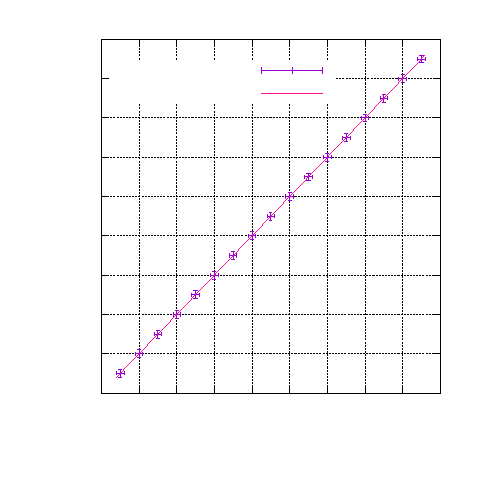
\includegraphics[width={223.20bp},height={216.00bp}]{Gráficas/RR01}}%
    \gplfronttext
  \end{picture}%
\endgroup

        		\caption{Ángulo de reflexión $\theta_r$ frente a ángulo de incidencia $\theta_i$ en aire-vidrio.}
        		\label{fig:AngReflAirVid}
        	\end{figure}

        	\begin{figure}[ht!]
            	\centering
            	% GNUPLOT: LaTeX picture with Postscript
\begingroup
  \makeatletter
  \providecommand\color[2][]{%
    \GenericError{(gnuplot) \space\space\space\@spaces}{%
      Package color not loaded in conjunction with
      terminal option `colourtext'%
    }{See the gnuplot documentation for explanation.%
    }{Either use 'blacktext' in gnuplot or load the package
      color.sty in LaTeX.}%
    \renewcommand\color[2][]{}%
  }%
  \providecommand\includegraphics[2][]{%
    \GenericError{(gnuplot) \space\space\space\@spaces}{%
      Package graphicx or graphics not loaded%
    }{See the gnuplot documentation for explanation.%
    }{The gnuplot epslatex terminal needs graphicx.sty or graphics.sty.}%
    \renewcommand\includegraphics[2][]{}%
  }%
  \providecommand\rotatebox[2]{#2}%
  \@ifundefined{ifGPcolor}{%
    \newif\ifGPcolor
    \GPcolorfalse
  }{}%
  \@ifundefined{ifGPblacktext}{%
    \newif\ifGPblacktext
    \GPblacktexttrue
  }{}%
  % define a \g@addto@macro without @ in the name:
  \let\gplgaddtomacro\g@addto@macro
  % define empty templates for all commands taking text:
  \gdef\gplbacktext{}%
  \gdef\gplfronttext{}%
  \makeatother
  \ifGPblacktext
    % no textcolor at all
    \def\colorrgb#1{}%
    \def\colorgray#1{}%
  \else
    % gray or color?
    \ifGPcolor
      \def\colorrgb#1{\color[rgb]{#1}}%
      \def\colorgray#1{\color[gray]{#1}}%
      \expandafter\def\csname LTw\endcsname{\color{white}}%
      \expandafter\def\csname LTb\endcsname{\color{black}}%
      \expandafter\def\csname LTa\endcsname{\color{black}}%
      \expandafter\def\csname LT0\endcsname{\color[rgb]{1,0,0}}%
      \expandafter\def\csname LT1\endcsname{\color[rgb]{0,1,0}}%
      \expandafter\def\csname LT2\endcsname{\color[rgb]{0,0,1}}%
      \expandafter\def\csname LT3\endcsname{\color[rgb]{1,0,1}}%
      \expandafter\def\csname LT4\endcsname{\color[rgb]{0,1,1}}%
      \expandafter\def\csname LT5\endcsname{\color[rgb]{1,1,0}}%
      \expandafter\def\csname LT6\endcsname{\color[rgb]{0,0,0}}%
      \expandafter\def\csname LT7\endcsname{\color[rgb]{1,0.3,0}}%
      \expandafter\def\csname LT8\endcsname{\color[rgb]{0.5,0.5,0.5}}%
    \else
      % gray
      \def\colorrgb#1{\color{black}}%
      \def\colorgray#1{\color[gray]{#1}}%
      \expandafter\def\csname LTw\endcsname{\color{white}}%
      \expandafter\def\csname LTb\endcsname{\color{black}}%
      \expandafter\def\csname LTa\endcsname{\color{black}}%
      \expandafter\def\csname LT0\endcsname{\color{black}}%
      \expandafter\def\csname LT1\endcsname{\color{black}}%
      \expandafter\def\csname LT2\endcsname{\color{black}}%
      \expandafter\def\csname LT3\endcsname{\color{black}}%
      \expandafter\def\csname LT4\endcsname{\color{black}}%
      \expandafter\def\csname LT5\endcsname{\color{black}}%
      \expandafter\def\csname LT6\endcsname{\color{black}}%
      \expandafter\def\csname LT7\endcsname{\color{black}}%
      \expandafter\def\csname LT8\endcsname{\color{black}}%
    \fi
  \fi
    \setlength{\unitlength}{0.0500bp}%
    \ifx\gptboxheight\undefined%
      \newlength{\gptboxheight}%
      \newlength{\gptboxwidth}%
      \newsavebox{\gptboxtext}%
    \fi%
    \setlength{\fboxrule}{0.5pt}%
    \setlength{\fboxsep}{1pt}%
\begin{picture}(4464.00,4320.00)%
    \gplgaddtomacro\gplbacktext{%
      \csname LTb\endcsname%%
      \put(682,704){\makebox(0,0)[r]{\strut{}$0$}}%
      \csname LTb\endcsname%%
      \put(682,1081){\makebox(0,0)[r]{\strut{}$10$}}%
      \csname LTb\endcsname%%
      \put(682,1458){\makebox(0,0)[r]{\strut{}$20$}}%
      \csname LTb\endcsname%%
      \put(682,1836){\makebox(0,0)[r]{\strut{}$30$}}%
      \csname LTb\endcsname%%
      \put(682,2213){\makebox(0,0)[r]{\strut{}$40$}}%
      \csname LTb\endcsname%%
      \put(682,2590){\makebox(0,0)[r]{\strut{}$50$}}%
      \csname LTb\endcsname%%
      \put(682,2967){\makebox(0,0)[r]{\strut{}$60$}}%
      \csname LTb\endcsname%%
      \put(682,3345){\makebox(0,0)[r]{\strut{}$70$}}%
      \csname LTb\endcsname%%
      \put(682,3722){\makebox(0,0)[r]{\strut{}$80$}}%
      \csname LTb\endcsname%%
      \put(682,4099){\makebox(0,0)[r]{\strut{}$90$}}%
      \csname LTb\endcsname%%
      \put(814,484){\makebox(0,0){\strut{}$0$}}%
      \csname LTb\endcsname%%
      \put(1175,484){\makebox(0,0){\strut{}$10$}}%
      \csname LTb\endcsname%%
      \put(1537,484){\makebox(0,0){\strut{}$20$}}%
      \csname LTb\endcsname%%
      \put(1898,484){\makebox(0,0){\strut{}$30$}}%
      \csname LTb\endcsname%%
      \put(2260,484){\makebox(0,0){\strut{}$40$}}%
      \csname LTb\endcsname%%
      \put(2621,484){\makebox(0,0){\strut{}$50$}}%
      \csname LTb\endcsname%%
      \put(2983,484){\makebox(0,0){\strut{}$60$}}%
      \csname LTb\endcsname%%
      \put(3344,484){\makebox(0,0){\strut{}$70$}}%
      \csname LTb\endcsname%%
      \put(3706,484){\makebox(0,0){\strut{}$80$}}%
      \csname LTb\endcsname%%
      \put(4067,484){\makebox(0,0){\strut{}$90$}}%
      \put(2343,1587){\makebox(0,0)[l]{\strut{}$\theta_r = m \theta_i + b$}}%
      \put(2343,1247){\makebox(0,0)[l]{\strut{}$m = 0,969 \pm 0,009$}}%
      \put(2343,908){\makebox(0,0)[l]{\strut{}$b = (0,2 \pm 0,7)$\textdegree}}%
    }%
    \gplgaddtomacro\gplfronttext{%
      \csname LTb\endcsname%%
      \put(209,2401){\rotatebox{-270}{\makebox(0,0){\strut{}$\theta_r$ (\textdegree)}}}%
      \put(2440,154){\makebox(0,0){\strut{}$\theta_i$ (\textdegree)}}%
      \csname LTb\endcsname%%
      \put(2217,3800){\makebox(0,0)[r]{\strut{}Datos exp.}}%
      \csname LTb\endcsname%%
      \put(2217,3580){\makebox(0,0)[r]{\strut{}Recta ajuste}}%
    }%
    \gplbacktext
    \put(0,0){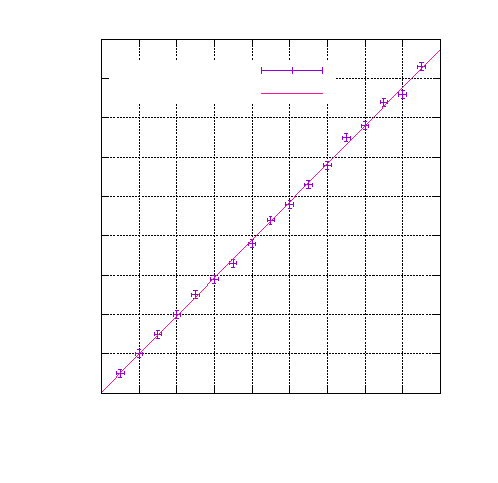
\includegraphics[width={223.20bp},height={216.00bp}]{Gráficas/RR04}}%
    \gplfronttext
  \end{picture}%
\endgroup

            	\caption{Ángulo de reflexión $\theta_r$ frente a ángulo de incidencia $\theta_i$ en aire-agua.}
        		\label{fig:AngReflAirAgu}
            \end{figure}
            
            Los errores de la pendiente de la recta ($m$) y de la ordenada del punto de corte con el eje vertical ($b$) son los indicados por el método empleado.

        \subsubsection{Comprobación de la ley de Snell o de la refracción}

            Se calculan en primer lugar los senos de los ángulos medidos en la primera parte de esta práctica. Los resultados se presentan en las tablas \ref{tab:SenAngAirVid} y \ref{tab:SenAngAirAgu}.

        	\begin{table}[!ht]
        		\centering
        		\caption{Seno de los ángulos de incidencia $\theta_i$, reflexión $\theta_r$ y refracción $\theta_t$ en aire-vidrio.}
        		
        		\resizebox{7.75cm}{!}{
        			
        			\vspace{0.1cm}
        			\begin{tabular}{ccc}
        				
        				\toprule % Para que nos pinte la linea superior horizontal de la tabla
        				
        				$\sin \theta_i$ & $\sin \theta_r$ & $\sin \theta_t$ \\
        				
        				\midrule % Para separar los encabezados del resto de la tabla
        				
        				$0,087 \pm 0,017$   & $0,087 \pm 0,017$     & $0,052 \pm 0,017$ \\
        				$0,174 \pm 0,017$  & $0,174 \pm 0,017$     & $0,105 \pm 0,017$ \\
        				$0,259 \pm 0,017$  & $0,259 \pm 0,017$     & $0,174 \pm 0,017$ \\
        				$0,342 \pm 0,016$  & $0,342 \pm 0,016$     & $0,225 \pm 0,017$ \\
        				$0,423 \pm 0,016$  & $0,423 \pm 0,016$     & $0,276 \pm 0,017$ \\
        				$0,500 \pm 0,015$  & $0,500 \pm 0,015$     & $0,326 \pm 0,017$ \\
        				$0,574 \pm 0,014$  & $0,574 \pm 0,014$     & $0,375 \pm 0,016$ \\
        				$0,643 \pm 0,013$  & $0,643 \pm 0,013$     & $0,423 \pm 0,016$ \\
        				$0,707 \pm 0,012$  & $0,707 \pm 0,012$     & $0,469 \pm 0,015$ \\
        				$0,766 \pm 0,011$  & $0,766 \pm 0,011$     & $0,515 \pm 0,015$ \\
        				$0,819 \pm 0,010$  & $0,819 \pm 0,010$     & $0,545 \pm 0,015$ \\
        				$0,866 \pm 0,009$  & $0,866 \pm 0,009$     & $0,574 \pm 0,014$ \\
        				$0,906 \pm 0,007$  & $0,906 \pm 0,007$     & $0,602 \pm 0,014$ \\
        				$0,940 \pm 0,006$  & $0,940 \pm 0,006$     & $0,629 \pm 0,014$ \\
        				$0,966 \pm 0,005$  & $0,966 \pm 0,005$     & $0,643 \pm 0,013$ \\
        				$0,985 \pm 0,003$  & $0,985 \pm 0,003$     & $0,656 \pm 0,013$ \\
        				$0,9962 \pm 0,0015$  & $0,9962 \pm 0,0015$     & $0,669 \pm 0,013$ \\
        				
        				\bottomrule 
        				
        			\end{tabular}
        			
        		}
        		
        		\label{tab:SenAngAirVid}
        	\end{table}

        	\begin{table}[!ht]
        		\centering
        		\caption{Seno de los ángulos de incidencia $\theta_i$, reflexión $\theta_r$ y refracción $\theta_t$ en aire-agua.}
        		
        		\resizebox{7.75cm}{!}{
        			
        			\vspace{0.1cm}
        			\begin{tabular}{ccc}
        				
        				\toprule % Para que nos pinte la linea superior horizontal de la tabla
        				
        				$\sin \theta_i$ & $\sin \theta_r$ & $\sin \theta_t$ \\
        				
        				\midrule % Para separar los encabezados del resto de la tabla
        				
        				$0,087 \pm 0,017$   & $0,087 \pm 0,017$     & $0,070 \pm 0,017$ \\
        				$0,174 \pm 0,017$  & $0,174 \pm 0,017$     & $0,122 \pm 0,017$ \\
        				$0,259 \pm 0,017$  & $0,259 \pm 0,017$     & $0,191 \pm 0,017$ \\
        				$0,342 \pm 0,016$  & $0,342 \pm 0,016$     & $0,242 \pm 0,017$ \\
        				$0,423 \pm 0,016$  & $0,423 \pm 0,016$     & $0,309 \pm 0,017$ \\
        				$0,500 \pm 0,015$  & $0,485 \pm 0,015$     & $0,358 \pm 0,016$ \\
        				$0,574 \pm 0,014$  & $0,545 \pm 0,015$     & $0,407 \pm 0,016$ \\
        				$0,643 \pm 0,013$  & $0,616 \pm 0,014$     & $0,454 \pm 0,016$ \\
        				$0,707 \pm 0,012$  & $0,695 \pm 0,013$     & $0,515 \pm 0,015$ \\
        				$0,766 \pm 0,011$  & $0,743 \pm 0,012$     & $0,559 \pm 0,014$ \\
        				$0,819 \pm 0,010$  & $0,799 \pm 0,011$     & $0,602 \pm 0,014$ \\
        				$0,866 \pm 0,009$  & $0,848 \pm 0,009$     & $0,602 \pm 0,014$ \\
        				$0,906 \pm 0,007$  & $0,906 \pm 0,007$     & $0,643 \pm 0,013$ \\
        				$0,940 \pm 0,006$  & $0,927 \pm 0,007$     & $0,669 \pm 0,013$ \\
        				$0,966 \pm 0,005$  & $0,961 \pm 0,005$     & $0,707 \pm 0,012$ \\
        				$0,985 \pm 0,003$  & $0,970 \pm 0,004$     & $0,731 \pm 0,012$ \\
        				$0,9962 \pm 0,0015$  & $0,993 \pm 0,002$     & $0,731 \pm 0,012$ \\
        				
        				\bottomrule 
        				
        			\end{tabular}
        			
        		}
        		
        		\label{tab:SenAngAirAgu}
        	\end{table}

            Los errores en la obtención de los senos de los ángulos se han obtenido por propagación lineal:
            
            $$ \epsilon_{\sin \theta} = | \cos \theta | \, \epsilon_\theta $$



            \underline{NOTA:} para realizar el cálculo de errores con funciones trigonométricas es preciso tener las unidades de los ángulos y sus respectivos errores en RADIANES.
            
            Se representan gráficamente los valores del seno del ángulo de refracción frente al seno del ángulo de incidencia, también para ambos experimentos. Se realiza una regresión lineal por ajuste de mínimos cuadrados para obtener la relación entre ambos valores (ver figuras \ref{fig:SenAngRefrAirVid} y \ref{fig:SenAngRefrAirAgu}).

        	\begin{figure}[ht!]
            	\centering
            	% GNUPLOT: LaTeX picture with Postscript
\begingroup
  \makeatletter
  \providecommand\color[2][]{%
    \GenericError{(gnuplot) \space\space\space\@spaces}{%
      Package color not loaded in conjunction with
      terminal option `colourtext'%
    }{See the gnuplot documentation for explanation.%
    }{Either use 'blacktext' in gnuplot or load the package
      color.sty in LaTeX.}%
    \renewcommand\color[2][]{}%
  }%
  \providecommand\includegraphics[2][]{%
    \GenericError{(gnuplot) \space\space\space\@spaces}{%
      Package graphicx or graphics not loaded%
    }{See the gnuplot documentation for explanation.%
    }{The gnuplot epslatex terminal needs graphicx.sty or graphics.sty.}%
    \renewcommand\includegraphics[2][]{}%
  }%
  \providecommand\rotatebox[2]{#2}%
  \@ifundefined{ifGPcolor}{%
    \newif\ifGPcolor
    \GPcolorfalse
  }{}%
  \@ifundefined{ifGPblacktext}{%
    \newif\ifGPblacktext
    \GPblacktexttrue
  }{}%
  % define a \g@addto@macro without @ in the name:
  \let\gplgaddtomacro\g@addto@macro
  % define empty templates for all commands taking text:
  \gdef\gplbacktext{}%
  \gdef\gplfronttext{}%
  \makeatother
  \ifGPblacktext
    % no textcolor at all
    \def\colorrgb#1{}%
    \def\colorgray#1{}%
  \else
    % gray or color?
    \ifGPcolor
      \def\colorrgb#1{\color[rgb]{#1}}%
      \def\colorgray#1{\color[gray]{#1}}%
      \expandafter\def\csname LTw\endcsname{\color{white}}%
      \expandafter\def\csname LTb\endcsname{\color{black}}%
      \expandafter\def\csname LTa\endcsname{\color{black}}%
      \expandafter\def\csname LT0\endcsname{\color[rgb]{1,0,0}}%
      \expandafter\def\csname LT1\endcsname{\color[rgb]{0,1,0}}%
      \expandafter\def\csname LT2\endcsname{\color[rgb]{0,0,1}}%
      \expandafter\def\csname LT3\endcsname{\color[rgb]{1,0,1}}%
      \expandafter\def\csname LT4\endcsname{\color[rgb]{0,1,1}}%
      \expandafter\def\csname LT5\endcsname{\color[rgb]{1,1,0}}%
      \expandafter\def\csname LT6\endcsname{\color[rgb]{0,0,0}}%
      \expandafter\def\csname LT7\endcsname{\color[rgb]{1,0.3,0}}%
      \expandafter\def\csname LT8\endcsname{\color[rgb]{0.5,0.5,0.5}}%
    \else
      % gray
      \def\colorrgb#1{\color{black}}%
      \def\colorgray#1{\color[gray]{#1}}%
      \expandafter\def\csname LTw\endcsname{\color{white}}%
      \expandafter\def\csname LTb\endcsname{\color{black}}%
      \expandafter\def\csname LTa\endcsname{\color{black}}%
      \expandafter\def\csname LT0\endcsname{\color{black}}%
      \expandafter\def\csname LT1\endcsname{\color{black}}%
      \expandafter\def\csname LT2\endcsname{\color{black}}%
      \expandafter\def\csname LT3\endcsname{\color{black}}%
      \expandafter\def\csname LT4\endcsname{\color{black}}%
      \expandafter\def\csname LT5\endcsname{\color{black}}%
      \expandafter\def\csname LT6\endcsname{\color{black}}%
      \expandafter\def\csname LT7\endcsname{\color{black}}%
      \expandafter\def\csname LT8\endcsname{\color{black}}%
    \fi
  \fi
    \setlength{\unitlength}{0.0500bp}%
    \ifx\gptboxheight\undefined%
      \newlength{\gptboxheight}%
      \newlength{\gptboxwidth}%
      \newsavebox{\gptboxtext}%
    \fi%
    \setlength{\fboxrule}{0.5pt}%
    \setlength{\fboxsep}{1pt}%
\begin{picture}(4464.00,4320.00)%
    \gplgaddtomacro\gplbacktext{%
      \csname LTb\endcsname%%
      \put(814,704){\makebox(0,0)[r]{\strut{}$0$}}%
      \csname LTb\endcsname%%
      \put(814,1189){\makebox(0,0)[r]{\strut{}$0.1$}}%
      \csname LTb\endcsname%%
      \put(814,1674){\makebox(0,0)[r]{\strut{}$0.2$}}%
      \csname LTb\endcsname%%
      \put(814,2159){\makebox(0,0)[r]{\strut{}$0.3$}}%
      \csname LTb\endcsname%%
      \put(814,2644){\makebox(0,0)[r]{\strut{}$0.4$}}%
      \csname LTb\endcsname%%
      \put(814,3129){\makebox(0,0)[r]{\strut{}$0.5$}}%
      \csname LTb\endcsname%%
      \put(814,3614){\makebox(0,0)[r]{\strut{}$0.6$}}%
      \csname LTb\endcsname%%
      \put(814,4099){\makebox(0,0)[r]{\strut{}$0.7$}}%
      \csname LTb\endcsname%%
      \put(946,484){\makebox(0,0){\strut{}$0$}}%
      \csname LTb\endcsname%%
      \put(1570,484){\makebox(0,0){\strut{}$0.2$}}%
      \csname LTb\endcsname%%
      \put(2194,484){\makebox(0,0){\strut{}$0.4$}}%
      \csname LTb\endcsname%%
      \put(2819,484){\makebox(0,0){\strut{}$0.6$}}%
      \csname LTb\endcsname%%
      \put(3443,484){\makebox(0,0){\strut{}$0.8$}}%
      \csname LTb\endcsname%%
      \put(4067,484){\makebox(0,0){\strut{}$1$}}%
      \put(2257,1553){\makebox(0,0)[l]{\strut{}$\sin \theta_t = m \sin \theta_i + b$}}%
      \put(2257,1281){\makebox(0,0)[l]{\strut{}$m = 0,676 \pm 0,003$}}%
      \put(2257,1010){\makebox(0,0)[l]{\strut{}$b = -0,008 \pm 0,004$}}%
    }%
    \gplgaddtomacro\gplfronttext{%
      \csname LTb\endcsname%%
      \put(209,2401){\rotatebox{-270}{\makebox(0,0){\strut{}$\sin \theta_t$}}}%
      \put(2506,154){\makebox(0,0){\strut{}$\sin \theta_i$}}%
      \csname LTb\endcsname%%
      \put(2374,3747){\makebox(0,0)[r]{\strut{}Datos exp.}}%
      \csname LTb\endcsname%%
      \put(2374,3527){\makebox(0,0)[r]{\strut{}Recta ajuste}}%
    }%
    \gplbacktext
    \put(0,0){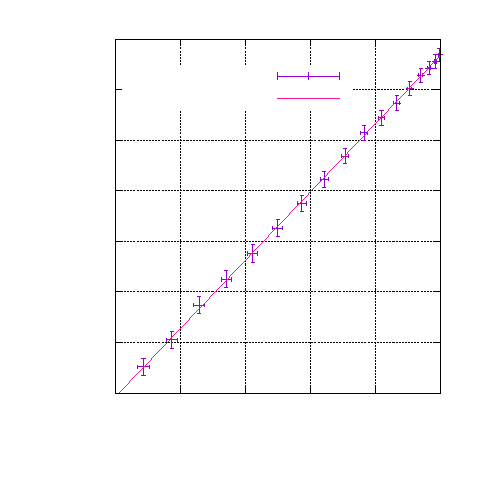
\includegraphics[width={223.20bp},height={216.00bp}]{Gráficas/RR02}}%
    \gplfronttext
  \end{picture}%
\endgroup

            	\caption{Seno del ángulo de refracción $\theta_t$ frente al seno del ángulo de incidencia $\theta_i$ en aire-vidrio.}
        		\label{fig:SenAngRefrAirVid}
            \end{figure}

        	\begin{figure}[ht!]
            	\centering
            	% GNUPLOT: LaTeX picture with Postscript
\begingroup
  \makeatletter
  \providecommand\color[2][]{%
    \GenericError{(gnuplot) \space\space\space\@spaces}{%
      Package color not loaded in conjunction with
      terminal option `colourtext'%
    }{See the gnuplot documentation for explanation.%
    }{Either use 'blacktext' in gnuplot or load the package
      color.sty in LaTeX.}%
    \renewcommand\color[2][]{}%
  }%
  \providecommand\includegraphics[2][]{%
    \GenericError{(gnuplot) \space\space\space\@spaces}{%
      Package graphicx or graphics not loaded%
    }{See the gnuplot documentation for explanation.%
    }{The gnuplot epslatex terminal needs graphicx.sty or graphics.sty.}%
    \renewcommand\includegraphics[2][]{}%
  }%
  \providecommand\rotatebox[2]{#2}%
  \@ifundefined{ifGPcolor}{%
    \newif\ifGPcolor
    \GPcolorfalse
  }{}%
  \@ifundefined{ifGPblacktext}{%
    \newif\ifGPblacktext
    \GPblacktexttrue
  }{}%
  % define a \g@addto@macro without @ in the name:
  \let\gplgaddtomacro\g@addto@macro
  % define empty templates for all commands taking text:
  \gdef\gplbacktext{}%
  \gdef\gplfronttext{}%
  \makeatother
  \ifGPblacktext
    % no textcolor at all
    \def\colorrgb#1{}%
    \def\colorgray#1{}%
  \else
    % gray or color?
    \ifGPcolor
      \def\colorrgb#1{\color[rgb]{#1}}%
      \def\colorgray#1{\color[gray]{#1}}%
      \expandafter\def\csname LTw\endcsname{\color{white}}%
      \expandafter\def\csname LTb\endcsname{\color{black}}%
      \expandafter\def\csname LTa\endcsname{\color{black}}%
      \expandafter\def\csname LT0\endcsname{\color[rgb]{1,0,0}}%
      \expandafter\def\csname LT1\endcsname{\color[rgb]{0,1,0}}%
      \expandafter\def\csname LT2\endcsname{\color[rgb]{0,0,1}}%
      \expandafter\def\csname LT3\endcsname{\color[rgb]{1,0,1}}%
      \expandafter\def\csname LT4\endcsname{\color[rgb]{0,1,1}}%
      \expandafter\def\csname LT5\endcsname{\color[rgb]{1,1,0}}%
      \expandafter\def\csname LT6\endcsname{\color[rgb]{0,0,0}}%
      \expandafter\def\csname LT7\endcsname{\color[rgb]{1,0.3,0}}%
      \expandafter\def\csname LT8\endcsname{\color[rgb]{0.5,0.5,0.5}}%
    \else
      % gray
      \def\colorrgb#1{\color{black}}%
      \def\colorgray#1{\color[gray]{#1}}%
      \expandafter\def\csname LTw\endcsname{\color{white}}%
      \expandafter\def\csname LTb\endcsname{\color{black}}%
      \expandafter\def\csname LTa\endcsname{\color{black}}%
      \expandafter\def\csname LT0\endcsname{\color{black}}%
      \expandafter\def\csname LT1\endcsname{\color{black}}%
      \expandafter\def\csname LT2\endcsname{\color{black}}%
      \expandafter\def\csname LT3\endcsname{\color{black}}%
      \expandafter\def\csname LT4\endcsname{\color{black}}%
      \expandafter\def\csname LT5\endcsname{\color{black}}%
      \expandafter\def\csname LT6\endcsname{\color{black}}%
      \expandafter\def\csname LT7\endcsname{\color{black}}%
      \expandafter\def\csname LT8\endcsname{\color{black}}%
    \fi
  \fi
    \setlength{\unitlength}{0.0500bp}%
    \ifx\gptboxheight\undefined%
      \newlength{\gptboxheight}%
      \newlength{\gptboxwidth}%
      \newsavebox{\gptboxtext}%
    \fi%
    \setlength{\fboxrule}{0.5pt}%
    \setlength{\fboxsep}{1pt}%
\begin{picture}(4464.00,4320.00)%
    \gplgaddtomacro\gplbacktext{%
      \csname LTb\endcsname%%
      \put(814,704){\makebox(0,0)[r]{\strut{}$0$}}%
      \csname LTb\endcsname%%
      \put(814,1128){\makebox(0,0)[r]{\strut{}$0.1$}}%
      \csname LTb\endcsname%%
      \put(814,1553){\makebox(0,0)[r]{\strut{}$0.2$}}%
      \csname LTb\endcsname%%
      \put(814,1977){\makebox(0,0)[r]{\strut{}$0.3$}}%
      \csname LTb\endcsname%%
      \put(814,2402){\makebox(0,0)[r]{\strut{}$0.4$}}%
      \csname LTb\endcsname%%
      \put(814,2826){\makebox(0,0)[r]{\strut{}$0.5$}}%
      \csname LTb\endcsname%%
      \put(814,3250){\makebox(0,0)[r]{\strut{}$0.6$}}%
      \csname LTb\endcsname%%
      \put(814,3675){\makebox(0,0)[r]{\strut{}$0.7$}}%
      \csname LTb\endcsname%%
      \put(814,4099){\makebox(0,0)[r]{\strut{}$0.8$}}%
      \csname LTb\endcsname%%
      \put(946,484){\makebox(0,0){\strut{}$0$}}%
      \csname LTb\endcsname%%
      \put(1570,484){\makebox(0,0){\strut{}$0.2$}}%
      \csname LTb\endcsname%%
      \put(2194,484){\makebox(0,0){\strut{}$0.4$}}%
      \csname LTb\endcsname%%
      \put(2819,484){\makebox(0,0){\strut{}$0.6$}}%
      \csname LTb\endcsname%%
      \put(3443,484){\makebox(0,0){\strut{}$0.8$}}%
      \csname LTb\endcsname%%
      \put(4067,484){\makebox(0,0){\strut{}$1$}}%
      \put(2257,1655){\makebox(0,0)[l]{\strut{}$\sin \theta_t = m \sin \theta_i + b$}}%
      \put(2257,1315){\makebox(0,0)[l]{\strut{}$m = 0,725 \pm 0,009$}}%
      \put(2257,976){\makebox(0,0)[l]{\strut{}$b = -0,002 \pm 0,011$}}%
    }%
    \gplgaddtomacro\gplfronttext{%
      \csname LTb\endcsname%%
      \put(209,2401){\rotatebox{-270}{\makebox(0,0){\strut{}$\sin \theta_t$}}}%
      \put(2506,154){\makebox(0,0){\strut{}$\sin \theta_i$}}%
      \csname LTb\endcsname%%
      \put(2374,3777){\makebox(0,0)[r]{\strut{}Datos exp.}}%
      \csname LTb\endcsname%%
      \put(2374,3557){\makebox(0,0)[r]{\strut{}Recta ajuste}}%
    }%
    \gplbacktext
    \put(0,0){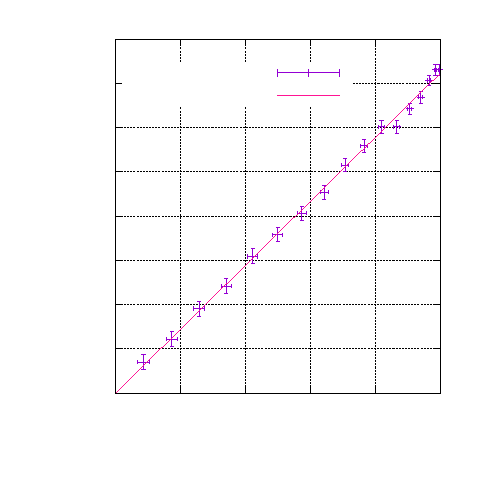
\includegraphics[width={223.20bp},height={216.00bp}]{Gráficas/RR05}}%
    \gplfronttext
  \end{picture}%
\endgroup

            	\caption{Seno del ángulo de refracción $\theta_t$ frente al seno del ángulo de incidencia $\theta_i$ en aire-agua.}
        		\label{fig:SenAngRefrAirAgu}
            \end{figure}

            Los errores de la pendiente de la recta ($m$) y de la ordenada del punto de corte con el eje vertical ($b$) son los indicados por el método empleado.
            
        \subsubsection{Aproximación paraxial o de Gauss}

            Tal y como se ha visto en el apartado \ref{cap:FunTeo}, para ángulos pequeños el ángulo de incidencia y el de refracción deberían ser proporcionales.
            
            Para comprobarlo, se representan ambos valores y para ambos experimentos en sendas gráficas. Se obtiene también la proporcionalidad (o pendiente) entre ambos ángulos a través de un ajuste lineal, para cuya realización se han utilizado únicamente los valores de los ángulos hasta 40\textdegree (ver figuras \ref{fig:AngRefrAirVid} y \ref{fig:AngRefrAirAgu}).
            
        	\begin{figure}[ht!]
            	\centering
            	% GNUPLOT: LaTeX picture with Postscript
\begingroup
  \makeatletter
  \providecommand\color[2][]{%
    \GenericError{(gnuplot) \space\space\space\@spaces}{%
      Package color not loaded in conjunction with
      terminal option `colourtext'%
    }{See the gnuplot documentation for explanation.%
    }{Either use 'blacktext' in gnuplot or load the package
      color.sty in LaTeX.}%
    \renewcommand\color[2][]{}%
  }%
  \providecommand\includegraphics[2][]{%
    \GenericError{(gnuplot) \space\space\space\@spaces}{%
      Package graphicx or graphics not loaded%
    }{See the gnuplot documentation for explanation.%
    }{The gnuplot epslatex terminal needs graphicx.sty or graphics.sty.}%
    \renewcommand\includegraphics[2][]{}%
  }%
  \providecommand\rotatebox[2]{#2}%
  \@ifundefined{ifGPcolor}{%
    \newif\ifGPcolor
    \GPcolorfalse
  }{}%
  \@ifundefined{ifGPblacktext}{%
    \newif\ifGPblacktext
    \GPblacktexttrue
  }{}%
  % define a \g@addto@macro without @ in the name:
  \let\gplgaddtomacro\g@addto@macro
  % define empty templates for all commands taking text:
  \gdef\gplbacktext{}%
  \gdef\gplfronttext{}%
  \makeatother
  \ifGPblacktext
    % no textcolor at all
    \def\colorrgb#1{}%
    \def\colorgray#1{}%
  \else
    % gray or color?
    \ifGPcolor
      \def\colorrgb#1{\color[rgb]{#1}}%
      \def\colorgray#1{\color[gray]{#1}}%
      \expandafter\def\csname LTw\endcsname{\color{white}}%
      \expandafter\def\csname LTb\endcsname{\color{black}}%
      \expandafter\def\csname LTa\endcsname{\color{black}}%
      \expandafter\def\csname LT0\endcsname{\color[rgb]{1,0,0}}%
      \expandafter\def\csname LT1\endcsname{\color[rgb]{0,1,0}}%
      \expandafter\def\csname LT2\endcsname{\color[rgb]{0,0,1}}%
      \expandafter\def\csname LT3\endcsname{\color[rgb]{1,0,1}}%
      \expandafter\def\csname LT4\endcsname{\color[rgb]{0,1,1}}%
      \expandafter\def\csname LT5\endcsname{\color[rgb]{1,1,0}}%
      \expandafter\def\csname LT6\endcsname{\color[rgb]{0,0,0}}%
      \expandafter\def\csname LT7\endcsname{\color[rgb]{1,0.3,0}}%
      \expandafter\def\csname LT8\endcsname{\color[rgb]{0.5,0.5,0.5}}%
    \else
      % gray
      \def\colorrgb#1{\color{black}}%
      \def\colorgray#1{\color[gray]{#1}}%
      \expandafter\def\csname LTw\endcsname{\color{white}}%
      \expandafter\def\csname LTb\endcsname{\color{black}}%
      \expandafter\def\csname LTa\endcsname{\color{black}}%
      \expandafter\def\csname LT0\endcsname{\color{black}}%
      \expandafter\def\csname LT1\endcsname{\color{black}}%
      \expandafter\def\csname LT2\endcsname{\color{black}}%
      \expandafter\def\csname LT3\endcsname{\color{black}}%
      \expandafter\def\csname LT4\endcsname{\color{black}}%
      \expandafter\def\csname LT5\endcsname{\color{black}}%
      \expandafter\def\csname LT6\endcsname{\color{black}}%
      \expandafter\def\csname LT7\endcsname{\color{black}}%
      \expandafter\def\csname LT8\endcsname{\color{black}}%
    \fi
  \fi
    \setlength{\unitlength}{0.0500bp}%
    \ifx\gptboxheight\undefined%
      \newlength{\gptboxheight}%
      \newlength{\gptboxwidth}%
      \newsavebox{\gptboxtext}%
    \fi%
    \setlength{\fboxrule}{0.5pt}%
    \setlength{\fboxsep}{1pt}%
\begin{picture}(4464.00,4320.00)%
    \gplgaddtomacro\gplbacktext{%
      \csname LTb\endcsname%%
      \put(682,704){\makebox(0,0)[r]{\strut{}$0$}}%
      \csname LTb\endcsname%%
      \put(682,1081){\makebox(0,0)[r]{\strut{}$10$}}%
      \csname LTb\endcsname%%
      \put(682,1458){\makebox(0,0)[r]{\strut{}$20$}}%
      \csname LTb\endcsname%%
      \put(682,1836){\makebox(0,0)[r]{\strut{}$30$}}%
      \csname LTb\endcsname%%
      \put(682,2213){\makebox(0,0)[r]{\strut{}$40$}}%
      \csname LTb\endcsname%%
      \put(682,2590){\makebox(0,0)[r]{\strut{}$50$}}%
      \csname LTb\endcsname%%
      \put(682,2967){\makebox(0,0)[r]{\strut{}$60$}}%
      \csname LTb\endcsname%%
      \put(682,3345){\makebox(0,0)[r]{\strut{}$70$}}%
      \csname LTb\endcsname%%
      \put(682,3722){\makebox(0,0)[r]{\strut{}$80$}}%
      \csname LTb\endcsname%%
      \put(682,4099){\makebox(0,0)[r]{\strut{}$90$}}%
      \csname LTb\endcsname%%
      \put(814,484){\makebox(0,0){\strut{}$0$}}%
      \csname LTb\endcsname%%
      \put(1175,484){\makebox(0,0){\strut{}$10$}}%
      \csname LTb\endcsname%%
      \put(1537,484){\makebox(0,0){\strut{}$20$}}%
      \csname LTb\endcsname%%
      \put(1898,484){\makebox(0,0){\strut{}$30$}}%
      \csname LTb\endcsname%%
      \put(2260,484){\makebox(0,0){\strut{}$40$}}%
      \csname LTb\endcsname%%
      \put(2621,484){\makebox(0,0){\strut{}$50$}}%
      \csname LTb\endcsname%%
      \put(2983,484){\makebox(0,0){\strut{}$60$}}%
      \csname LTb\endcsname%%
      \put(3344,484){\makebox(0,0){\strut{}$70$}}%
      \csname LTb\endcsname%%
      \put(3706,484){\makebox(0,0){\strut{}$80$}}%
      \csname LTb\endcsname%%
      \put(4067,484){\makebox(0,0){\strut{}$90$}}%
      \put(1248,3156){\makebox(0,0)[l]{\strut{}$\theta_t = m \theta_i$}}%
      \put(1248,2779){\makebox(0,0)[l]{\strut{}$m = 0,636 \pm 0,012$}}%
    }%
    \gplgaddtomacro\gplfronttext{%
      \csname LTb\endcsname%%
      \put(209,2401){\rotatebox{-270}{\makebox(0,0){\strut{}$\theta_t$ (\textdegree)}}}%
      \put(2440,154){\makebox(0,0){\strut{}$\theta_i$ (\textdegree)}}%
      \csname LTb\endcsname%%
      \put(2217,3800){\makebox(0,0)[r]{\strut{}Datos exp.}}%
      \csname LTb\endcsname%%
      \put(2217,3580){\makebox(0,0)[r]{\strut{}Recta ajuste}}%
    }%
    \gplbacktext
    \put(0,0){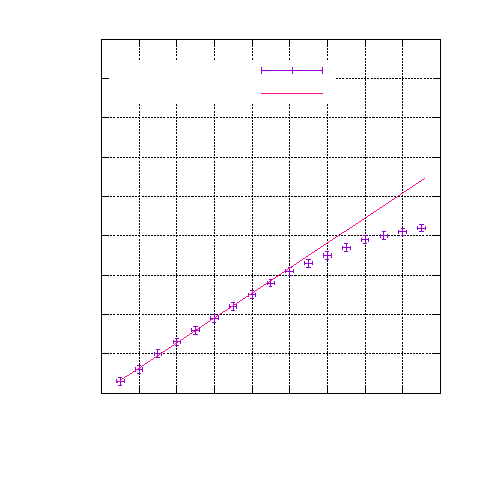
\includegraphics[width={223.20bp},height={216.00bp}]{Gráficas/RR03}}%
    \gplfronttext
  \end{picture}%
\endgroup

            	\caption{Ángulo de refracción $\theta_t$ frente a ángulo de incidencia $\theta_i$ en aire-vidrio.}
                \label{fig:AngRefrAirVid}
            \end{figure}

            \begin{figure}[ht!]
            	\centering
            	% GNUPLOT: LaTeX picture with Postscript
\begingroup
  \makeatletter
  \providecommand\color[2][]{%
    \GenericError{(gnuplot) \space\space\space\@spaces}{%
      Package color not loaded in conjunction with
      terminal option `colourtext'%
    }{See the gnuplot documentation for explanation.%
    }{Either use 'blacktext' in gnuplot or load the package
      color.sty in LaTeX.}%
    \renewcommand\color[2][]{}%
  }%
  \providecommand\includegraphics[2][]{%
    \GenericError{(gnuplot) \space\space\space\@spaces}{%
      Package graphicx or graphics not loaded%
    }{See the gnuplot documentation for explanation.%
    }{The gnuplot epslatex terminal needs graphicx.sty or graphics.sty.}%
    \renewcommand\includegraphics[2][]{}%
  }%
  \providecommand\rotatebox[2]{#2}%
  \@ifundefined{ifGPcolor}{%
    \newif\ifGPcolor
    \GPcolorfalse
  }{}%
  \@ifundefined{ifGPblacktext}{%
    \newif\ifGPblacktext
    \GPblacktexttrue
  }{}%
  % define a \g@addto@macro without @ in the name:
  \let\gplgaddtomacro\g@addto@macro
  % define empty templates for all commands taking text:
  \gdef\gplbacktext{}%
  \gdef\gplfronttext{}%
  \makeatother
  \ifGPblacktext
    % no textcolor at all
    \def\colorrgb#1{}%
    \def\colorgray#1{}%
  \else
    % gray or color?
    \ifGPcolor
      \def\colorrgb#1{\color[rgb]{#1}}%
      \def\colorgray#1{\color[gray]{#1}}%
      \expandafter\def\csname LTw\endcsname{\color{white}}%
      \expandafter\def\csname LTb\endcsname{\color{black}}%
      \expandafter\def\csname LTa\endcsname{\color{black}}%
      \expandafter\def\csname LT0\endcsname{\color[rgb]{1,0,0}}%
      \expandafter\def\csname LT1\endcsname{\color[rgb]{0,1,0}}%
      \expandafter\def\csname LT2\endcsname{\color[rgb]{0,0,1}}%
      \expandafter\def\csname LT3\endcsname{\color[rgb]{1,0,1}}%
      \expandafter\def\csname LT4\endcsname{\color[rgb]{0,1,1}}%
      \expandafter\def\csname LT5\endcsname{\color[rgb]{1,1,0}}%
      \expandafter\def\csname LT6\endcsname{\color[rgb]{0,0,0}}%
      \expandafter\def\csname LT7\endcsname{\color[rgb]{1,0.3,0}}%
      \expandafter\def\csname LT8\endcsname{\color[rgb]{0.5,0.5,0.5}}%
    \else
      % gray
      \def\colorrgb#1{\color{black}}%
      \def\colorgray#1{\color[gray]{#1}}%
      \expandafter\def\csname LTw\endcsname{\color{white}}%
      \expandafter\def\csname LTb\endcsname{\color{black}}%
      \expandafter\def\csname LTa\endcsname{\color{black}}%
      \expandafter\def\csname LT0\endcsname{\color{black}}%
      \expandafter\def\csname LT1\endcsname{\color{black}}%
      \expandafter\def\csname LT2\endcsname{\color{black}}%
      \expandafter\def\csname LT3\endcsname{\color{black}}%
      \expandafter\def\csname LT4\endcsname{\color{black}}%
      \expandafter\def\csname LT5\endcsname{\color{black}}%
      \expandafter\def\csname LT6\endcsname{\color{black}}%
      \expandafter\def\csname LT7\endcsname{\color{black}}%
      \expandafter\def\csname LT8\endcsname{\color{black}}%
    \fi
  \fi
    \setlength{\unitlength}{0.0500bp}%
    \ifx\gptboxheight\undefined%
      \newlength{\gptboxheight}%
      \newlength{\gptboxwidth}%
      \newsavebox{\gptboxtext}%
    \fi%
    \setlength{\fboxrule}{0.5pt}%
    \setlength{\fboxsep}{1pt}%
\begin{picture}(4464.00,4320.00)%
    \gplgaddtomacro\gplbacktext{%
      \csname LTb\endcsname%%
      \put(682,704){\makebox(0,0)[r]{\strut{}$0$}}%
      \csname LTb\endcsname%%
      \put(682,1081){\makebox(0,0)[r]{\strut{}$10$}}%
      \csname LTb\endcsname%%
      \put(682,1458){\makebox(0,0)[r]{\strut{}$20$}}%
      \csname LTb\endcsname%%
      \put(682,1836){\makebox(0,0)[r]{\strut{}$30$}}%
      \csname LTb\endcsname%%
      \put(682,2213){\makebox(0,0)[r]{\strut{}$40$}}%
      \csname LTb\endcsname%%
      \put(682,2590){\makebox(0,0)[r]{\strut{}$50$}}%
      \csname LTb\endcsname%%
      \put(682,2967){\makebox(0,0)[r]{\strut{}$60$}}%
      \csname LTb\endcsname%%
      \put(682,3345){\makebox(0,0)[r]{\strut{}$70$}}%
      \csname LTb\endcsname%%
      \put(682,3722){\makebox(0,0)[r]{\strut{}$80$}}%
      \csname LTb\endcsname%%
      \put(682,4099){\makebox(0,0)[r]{\strut{}$90$}}%
      \csname LTb\endcsname%%
      \put(814,484){\makebox(0,0){\strut{}$0$}}%
      \csname LTb\endcsname%%
      \put(1175,484){\makebox(0,0){\strut{}$10$}}%
      \csname LTb\endcsname%%
      \put(1537,484){\makebox(0,0){\strut{}$20$}}%
      \csname LTb\endcsname%%
      \put(1898,484){\makebox(0,0){\strut{}$30$}}%
      \csname LTb\endcsname%%
      \put(2260,484){\makebox(0,0){\strut{}$40$}}%
      \csname LTb\endcsname%%
      \put(2621,484){\makebox(0,0){\strut{}$50$}}%
      \csname LTb\endcsname%%
      \put(2983,484){\makebox(0,0){\strut{}$60$}}%
      \csname LTb\endcsname%%
      \put(3344,484){\makebox(0,0){\strut{}$70$}}%
      \csname LTb\endcsname%%
      \put(3706,484){\makebox(0,0){\strut{}$80$}}%
      \csname LTb\endcsname%%
      \put(4067,484){\makebox(0,0){\strut{}$90$}}%
      \put(1248,3156){\makebox(0,0)[l]{\strut{}$\theta_t = m \theta_i$}}%
      \put(1248,2779){\makebox(0,0)[l]{\strut{}$m = 0,679 \pm 0,012$}}%
    }%
    \gplgaddtomacro\gplfronttext{%
      \csname LTb\endcsname%%
      \put(209,2401){\rotatebox{-270}{\makebox(0,0){\strut{}$\theta_t$ (\textdegree)}}}%
      \put(2440,154){\makebox(0,0){\strut{}$\theta_i$ (\textdegree)}}%
      \csname LTb\endcsname%%
      \put(2217,3800){\makebox(0,0)[r]{\strut{}Datos exp.}}%
      \csname LTb\endcsname%%
      \put(2217,3580){\makebox(0,0)[r]{\strut{}Recta ajuste}}%
    }%
    \gplbacktext
    \put(0,0){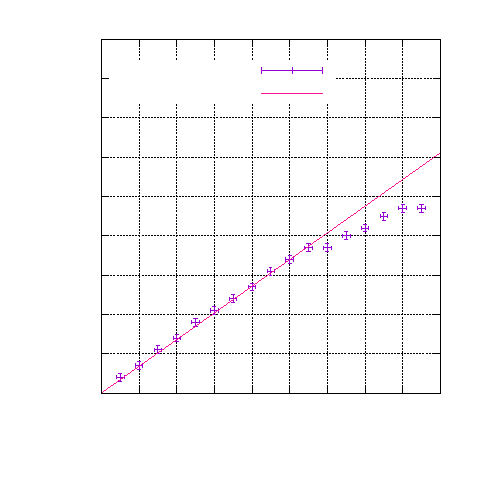
\includegraphics[width={223.20bp},height={216.00bp}]{Gráficas/RR06}}%
    \gplfronttext
  \end{picture}%
\endgroup

            	\caption{Ángulo de refracción $\theta_t$ frente a ángulo de incidencia $\theta_i$ en aire-agua.}
                \label{fig:AngRefrAirAgu}
            \end{figure}            

            El error de las pendientes de las rectas ($m$) es el indicado por el método empleado.

    \subsection{Ángulo límite}
	
	    Para encontrar este valor, se incide con el láser desde la parte curva de la cubeta (vidrio o agua) con ángulos para los que haya refracción hacia el aire. Se va aumentando el ángulo de incidencia hasta que deje de aparecer el rayo por la parte recta de la cubeta.
	    
	    Se repite la operación, pero ahora comenzando por ángulos de incidencia para los que no haya refracción hacia el aire. Se va disminuyendo el ángulo de incidencia hasta que aparezca el rayo transmitido por la parte recta de la cubeta.

            Los resultados obtenidos se presentan en las tablas \ref{tab:AngLimVidAir} y \ref{tab:AngLimAguAir}.

            \begin{table}[!ht]
            	\centering
        		\caption{Ángulos de incidencia $\theta_i$ desde el vidrio al aire en torno al ángulo límite.}
            		
        		\resizebox{7.75cm}{!}{
            			
            		\vspace{0.1cm}
            		\begin{tabular}{ccc}
            				
            			\toprule % Para que nos pinte la linea superior horizontal de la tabla
            				
            			$\theta_i$ (\textdegree) & Transmisión & No transmisión \\
            				
            			\midrule % Para separar los encabezados del resto de la tabla
            				
            			$38 \pm 1$ & X & - \\
            			$39 \pm 1$ & X & - \\
            			$40 \pm 1$ & X & - \\        			
            			$41 \pm 1$ & X & - \\
            			$42 \pm 1$ & - & X \\
            			$43 \pm 1$ & - & X \\
            			$44 \pm 1$ & - & X \\
            			$45 \pm 1$ & - & X \\
            				
            			\bottomrule 
            				
            		\end{tabular}
            			
            	}
            		
        		\label{tab:AngLimVidAir}
        	\end{table}

                \begin{table}[!ht]
                	\centering
            		\caption{Ángulos de incidencia $\theta_i$ desde el agua al aire en torno al ángulo límite.}
                		
            		\resizebox{7.75cm}{!}{
                			
                		\vspace{0.1cm}
                		\begin{tabular}{ccc}
                				
                			\toprule % Para que nos pinte la linea superior horizontal de la tabla
                				
                			$\theta_i$ (\textdegree) & Transmisión & No transmisión \\
                				
                			\midrule % Para separar los encabezados del resto de la tabla
                				
                			$43 \pm 1$ & X & - \\
                			$44 \pm 1$ & X & - \\
                			$45 \pm 1$ & X & - \\        			
                			$46 \pm 1$ & X & - \\
                			$47 \pm 1$ & X & - \\
                			$48 \pm 1$ & - & X \\
                			$49 \pm 1$ & - & X \\
                			$50 \pm 1$ & - & X \\
                				
                			\bottomrule 
                				
                		\end{tabular}
                			
                	}
                		
            		\label{tab:AngLimAguAir}
            	\end{table}  


     
	    Se toma el ángulo límite como la media entre esos dos valores, que deberán estar -y están- muy cercanos.
	    
	 El valor del ángulo límite para el caso de transmisión de vidrio a aire se puede considerar entonces:
        
        $$ \theta_{l_{vidrio-aire}} = (41,5 \pm 1,0)\text{\textdegree}$$
        
        El valor del ángulo límite para el caso de transmisión de agua a aire se puede considerar entonces:
        
        $$ \theta_{l_{agua-aire}} = (47,5 \pm 1,0)\text{\textdegree} $$	

        Los errores aplicados son los debidos al dispositivo experimental, ya indicados en el apartado \ref{cap:MedAngIncReflRefr}.
	
	\section{Conclusiones}

    % Explicar los resultados. Evaluar coincidencia o no de los resultados con la teoría conocida.
    
    % No se juzgan los resultados ni se dan opiniones..
    
    Se analiza a continuación si los resultados obtenidos sirven para comprobar las leyes de la reflexión y la refracción, para constatar la existencia de la reflexión total y para determinar el índice de refracción del vidrio y del agua respecto del aire.
    
    \begin{itemize}

        \item \textbf{Ley de la reflexión:} las pendientes de las rectas de las figuras \ref{fig:AngReflAirVid} y \ref{fig:AngReflAirAgu} son prácticamente la unidad. Por lo tanto, el ángulo reflejado es igual al ángulo de incidencia.
        
        \item \textbf{Ley de la refracción:} la pendiente de la recta de la figura \ref{fig:SenAngRefrAirVid} es $0,676 \pm 0,003$. El índice de refracción del vidrio es la inversa de esta pendiente, por lo tanto:
        $$ n_v = \frac{1}{m_v} = \frac{1}{0,676 \pm 0,003} = 1,479 \pm 0,007 $$        
        La diferencia entre este valor y el que se encuentra en la literatura (1,45) está dentro del margen de error del experimento.

        La pendiente de la recta de la figura \ref{fig:SenAngRefrAirAgu} es $0,725 \pm 0,009$. El índice de refracción del agua es la inversa de esta pendiente, por lo tanto:
        $$ n_a = \frac{1}{m_a} = \frac{1}{0,725 \pm 0,009} = 1,379 \pm 0,017 $$
        La diferencia entre este valor y el que se encuentra en la literatura (1,33) está dentro del margen de error del experimento.

        \item \textbf{Aproximación paraxial o de Gauss:} la pendiente de la recta de la figura \ref{fig:AngRefrAirVid} es $0,636 \pm 0,012$. Esto corresponde a un índice de refracción para el vidrio de:        
        $$ n_v = \frac{1}{m_v} = \frac{1}{0,636 \pm 0,012} = 1,57 \pm 0,03 $$
        La diferencia entre la aproximación paraxial y la ley de Snell está dentro del margen de error de la medida.

        La pendiente de la recta de la figura \ref{fig:AngRefrAirAgu} es $0,679 \pm 0,012$. Esto corresponde a un índice de refracción para el agua de:        
        $$ n_a = \frac{1}{m_a} = \frac{1}{0,679 \pm 0,012} = 1,47 \pm 0,03 $$
        La diferencia entre la aproximación paraxial y la ley de Snell está dentro del margen de error de la medida.

        \item \textbf{Reflexión total y ángulo límite:} el ángulo límite se produce cuando el ángulo de refracción tiende a 90\textdegree. Por lo tanto:

        $$ \sin \theta_l = \frac{1}{n} \sin 90 \text{\textdegree} \rightarrow n = \frac{1}{\sin \theta_l} $$
        
        En el caso de la superficie vidrio-aire tenemos:
        $$ \theta_{l_v} = (41,5 \pm 1,0) \textbf{\textdegree} \rightarrow \sin \theta_{l_v} = 0,663 \pm 0,013 $$
        $$ n_v = \frac{1}{0,663 \pm 0,013} = 1,51 \pm 0,03 $$
        El resultado obtenido para $n_v$ por este método coincide con el obtenido por la ley de Snell, dentro de los márgenes de error de la medida.

        En el caso de la superficie vidrio-agua tenemos:
        $$ \theta_{l_a} = (47,5 \pm 1,0) \textbf{\textdegree} \rightarrow \sin \theta_{l_a} = 0,737 \pm 0,012 $$
        $$ n_a = \frac{1}{0,737 \pm 0,012} = 1,36 \pm 0,02 $$
        El resultado obtenido para $n_a$ por este método coincide con el obtenido por la ley de Snell, dentro de los márgenes de error de la medida.      

        

    \end{itemize}

    \ul{En consecuencia estos experimentos son adecuados para estudiar las leyes elementales de la \'Optica}.\\

    \underline{NOTA:} la propagación de errores empleada en este apartado para el cálculo de $n$ y $\sin \theta$ es lineal, y sus valores son:

    $$ \epsilon_n = \left| - \frac{1}{m^2} \right| \epsilon_m $$
    $$ \epsilon_{\sin \theta} = | \cos \theta | \epsilon_{\theta} $$
 
%	\section{Cuestiones}
	
%	\section{Bibliografía}
	
    \bibliographystyle{babunsrt}

    \bibliography{Bibliografia.bib}	
	
	
	
\end{document}